\chapter{Perancangan}
\label{chap:perancangan}

\section{Perancangan Kelas Akibat Kurikulum 2018}

Pada subbab ini akan menjelaskan perancangan kelas akibat kurikulum 2018 dari hasil analisis pada subbab \ref{subbab:analisissiamodels} \& \ref{subbab:analisisifstudentportal}. Diagram kelas akibat kurikulum 2018 dibagi menjadi beberapa bagian yang dapat dilihat pada gambar \ref{fig:siamodels_class_2018} untuk diagram kelas SIAModels yang berubah pada kelas \texttt{Nilai} dan untuk diagram kelas lengkapnya dapat dilihat pada gambar \ref{fig:2_siamodels_class}. Gambar \ref{fig:siamodels_class_2018_kurikulum_1}, \ref{fig:siamodels_class_2018_kurikulum_2}, \ref{fig:siamodels_class_2018_kurikulum_3}, \ref{fig:siamodels_class_2018_kurikulum_4}, dan \ref{fig:siamodels_class_2018_kurikulum_5} untuk diagram kelas yang merepresentasikan mata kuliah pada kurikulum 2018. Deskripsi kelas berserta fungsi dari diagram kelas tersebut adalah sebagai berikut:

\begin{figure}[H]
\centering
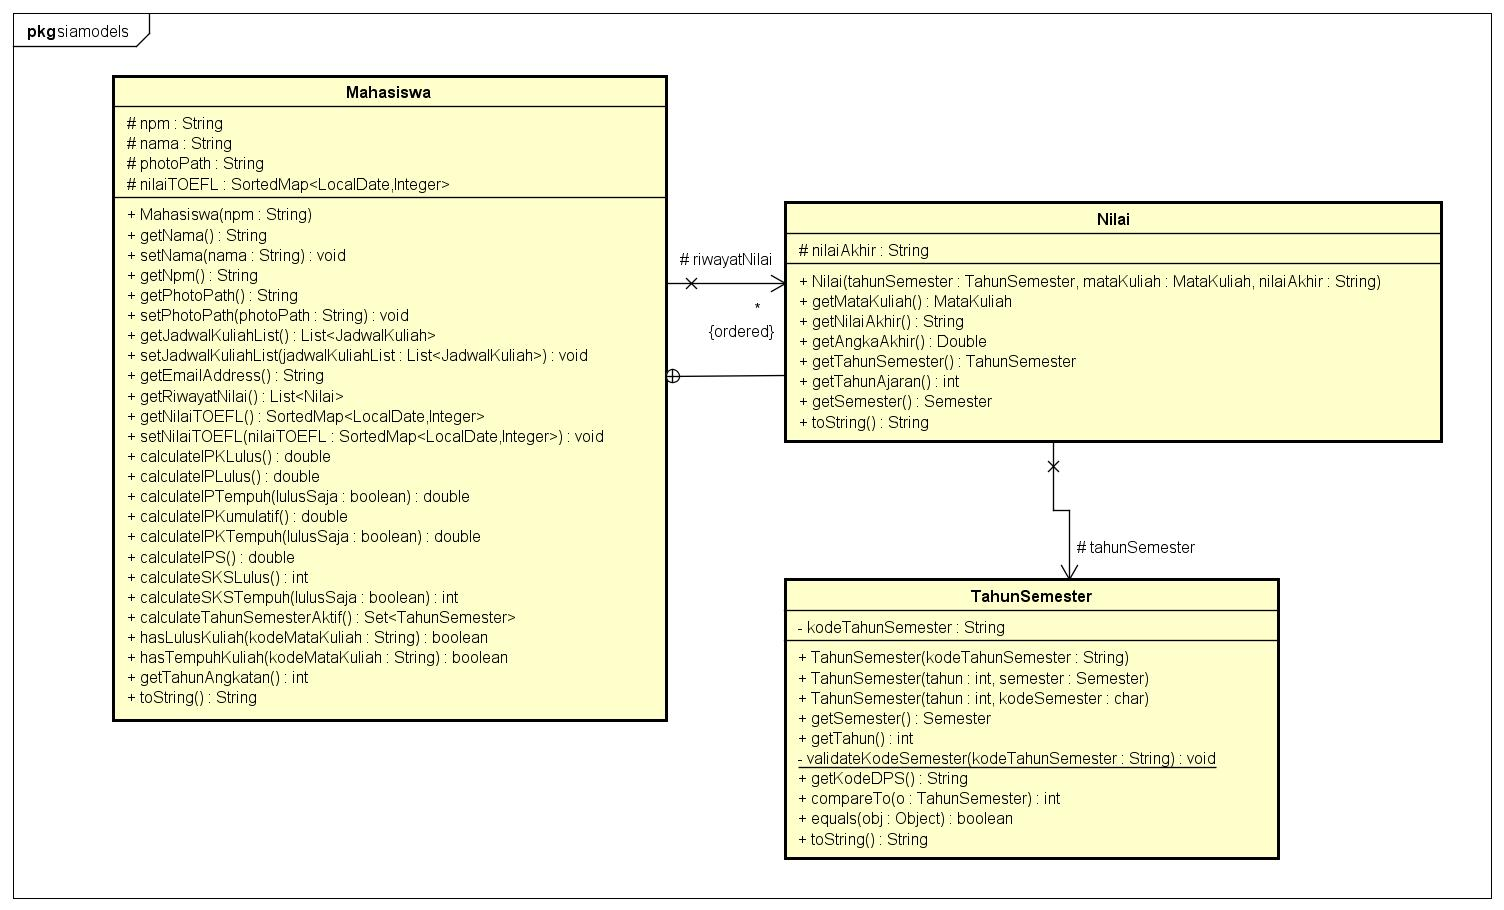
\includegraphics[scale=0.15]{Gambar/class-diagram-siamodels-new}
\caption{Diagram Kelas SIAModels Bagian \texttt{Nilai}}
\label{fig:siamodels_class_2018}
\end{figure}

\begin{figure}[H]
\centering
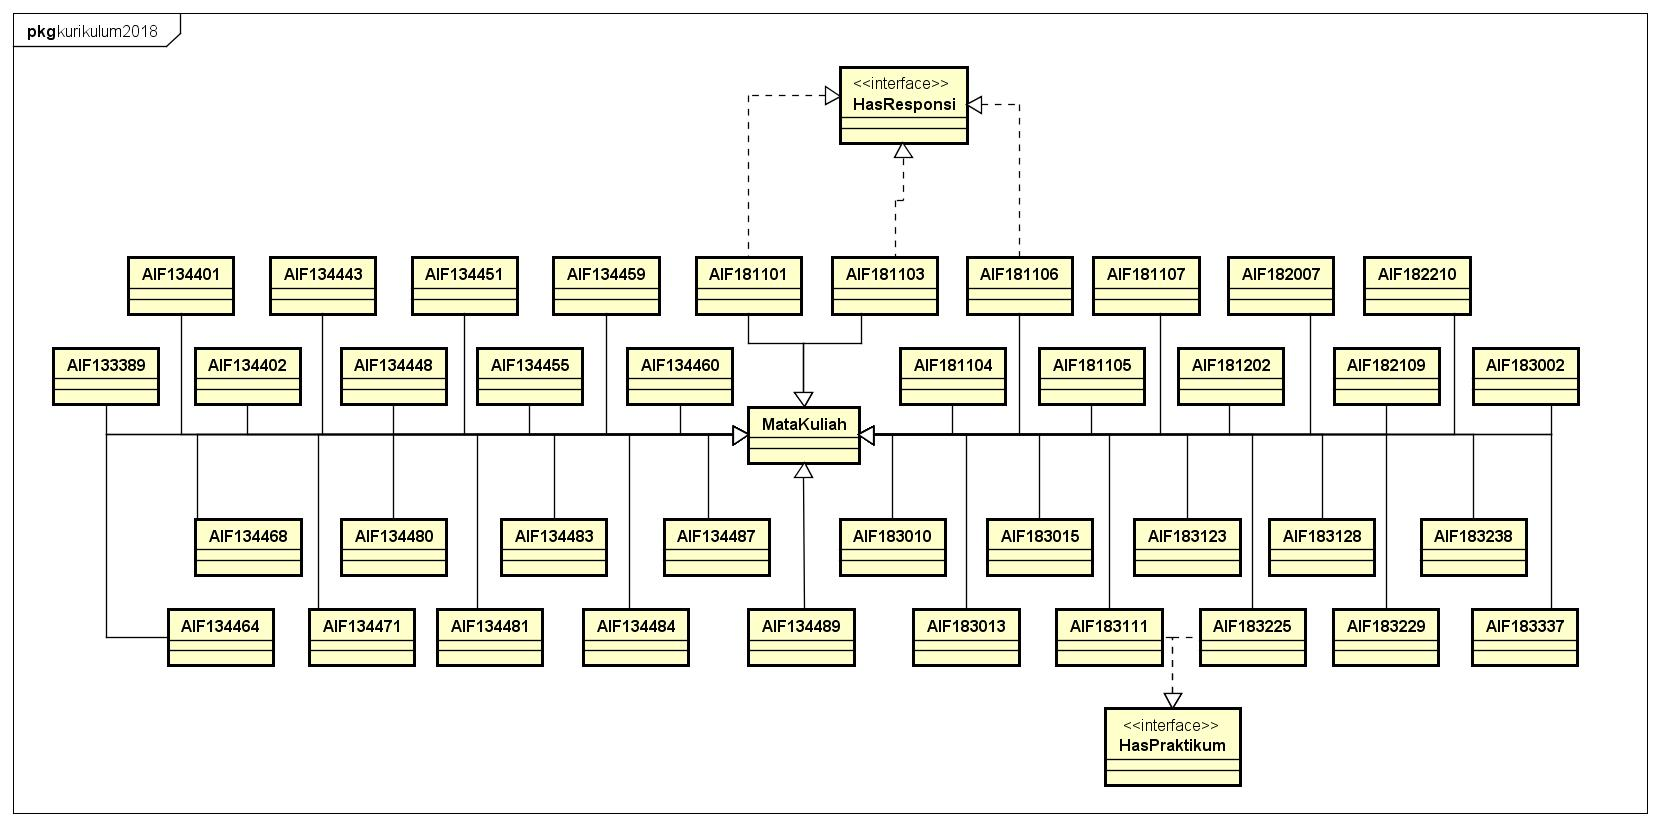
\includegraphics[scale=0.4]{Gambar/class-diagram-siamodels-mk-kurikulum-2018-2}
\caption{Diagram Kelas SIAModels \textit{Package} \texttt{kurikulum2018} 1}
\label{fig:siamodels_class_2018_kurikulum_1}
\end{figure}

\begin{figure}[H]
\centering
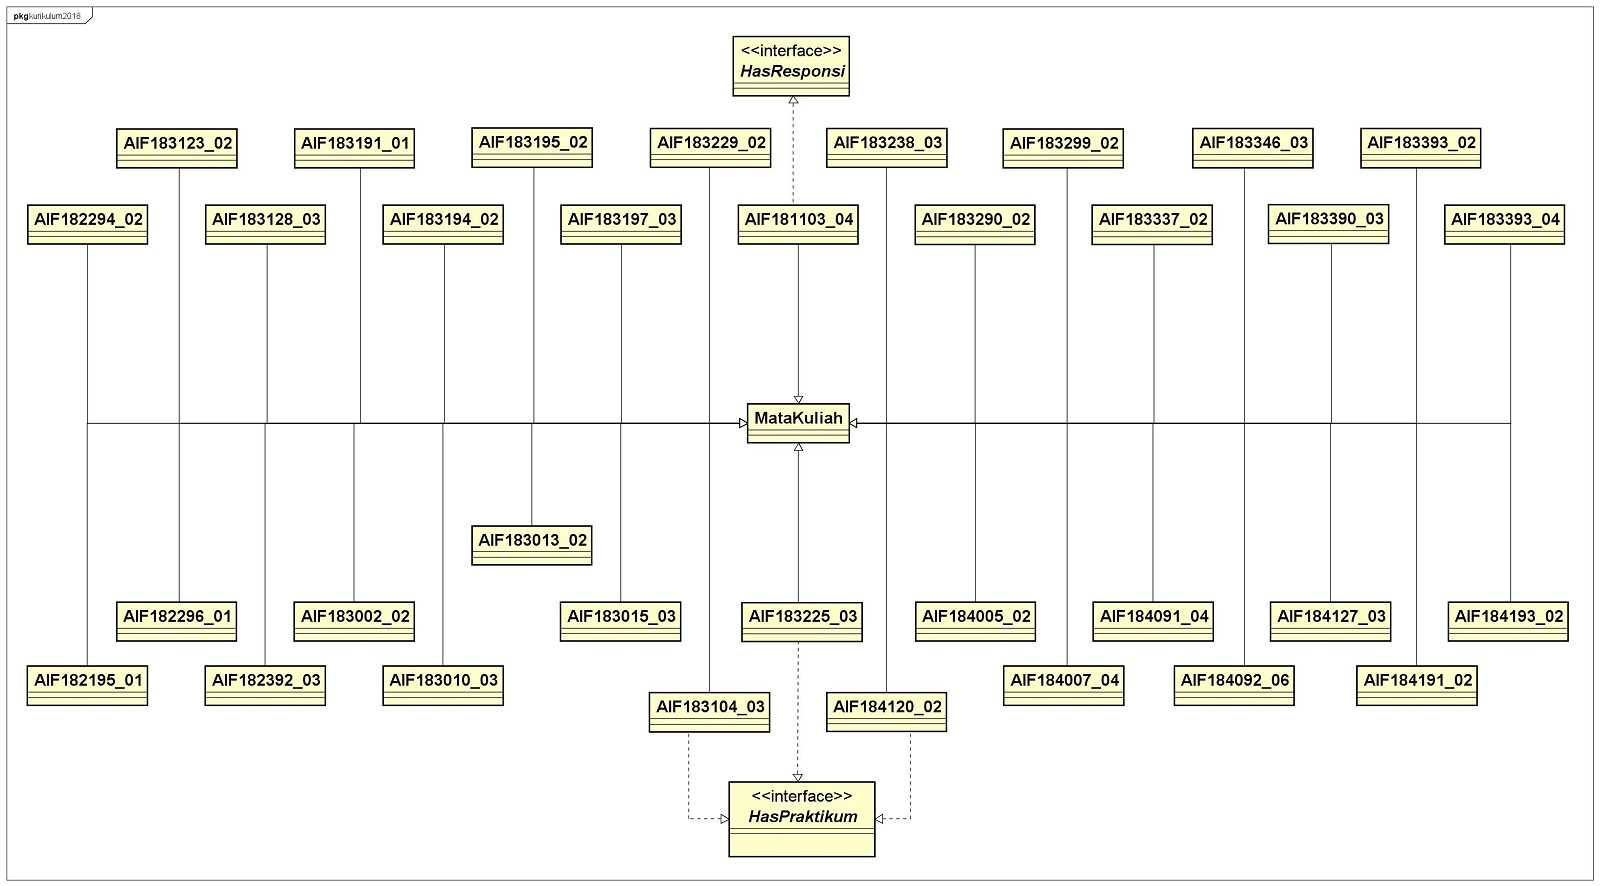
\includegraphics[scale=0.4]{Gambar/class-diagram-siamodels-mk-kurikulum-2018-1}
\caption{Diagram Kelas SIAModels \textit{Package} \texttt{kurikulum2018} 2}
\label{fig:siamodels_class_2018_kurikulum_2}
\end{figure}

\begin{figure}[H]
\centering
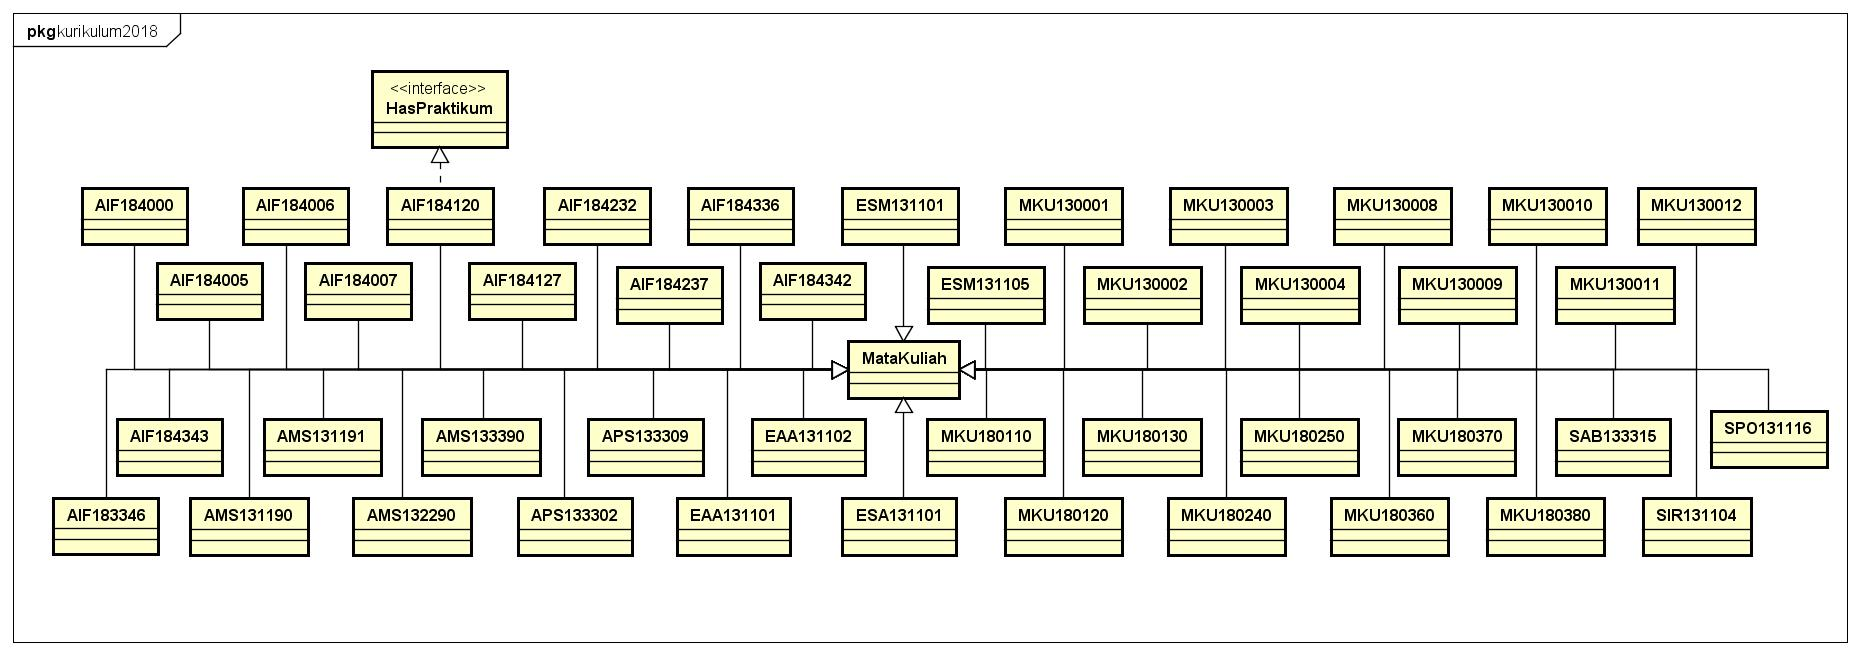
\includegraphics[scale=0.15]{Gambar/class-diagram-siamodels-mk-kurikulum-2018-3}
\caption{Diagram Kelas SIAModels \textit{Package} \texttt{kurikulum2018} 3}
\label{fig:siamodels_class_2018_kurikulum_3}
\end{figure}

\begin{figure}[H]
\centering
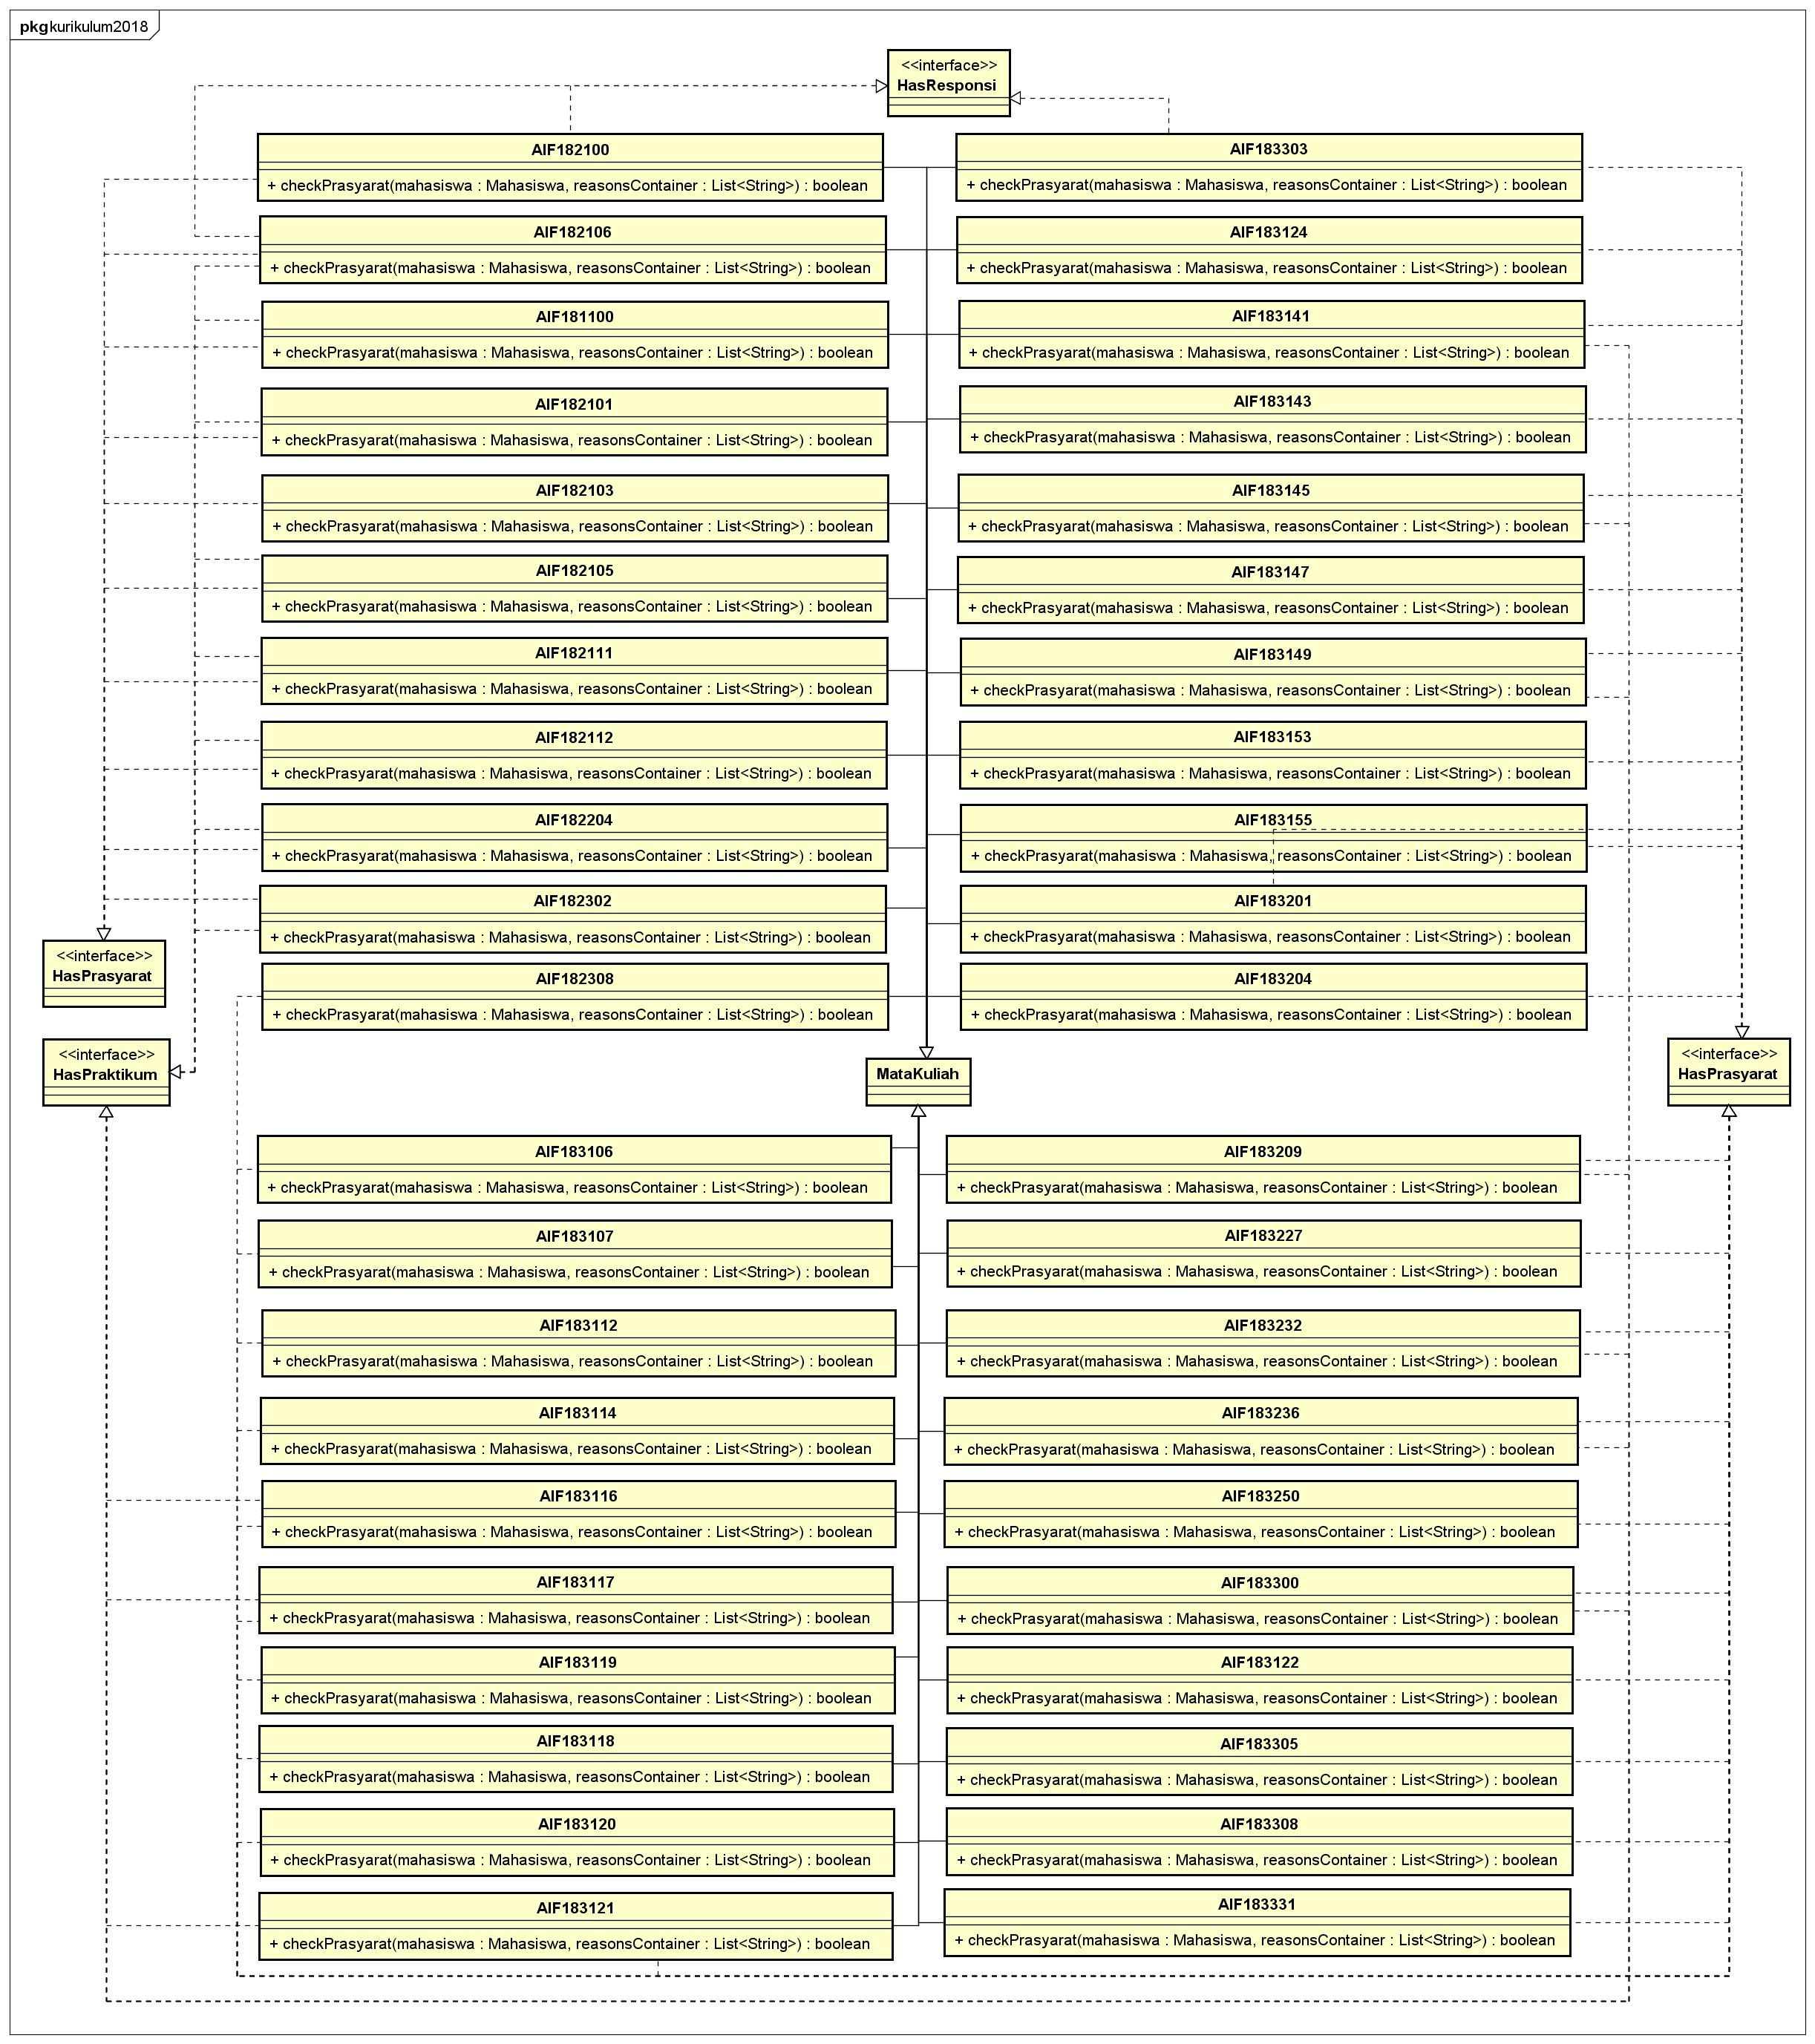
\includegraphics[scale=0.135]{Gambar/class-diagram-siamodels-mk-kurikulum-2018-4}
\caption{Diagram Kelas SIAModels \textit{Package} \texttt{kurikulum2018} 4}
\label{fig:siamodels_class_2018_kurikulum_4}
\end{figure}

\begin{figure}[H]
\centering
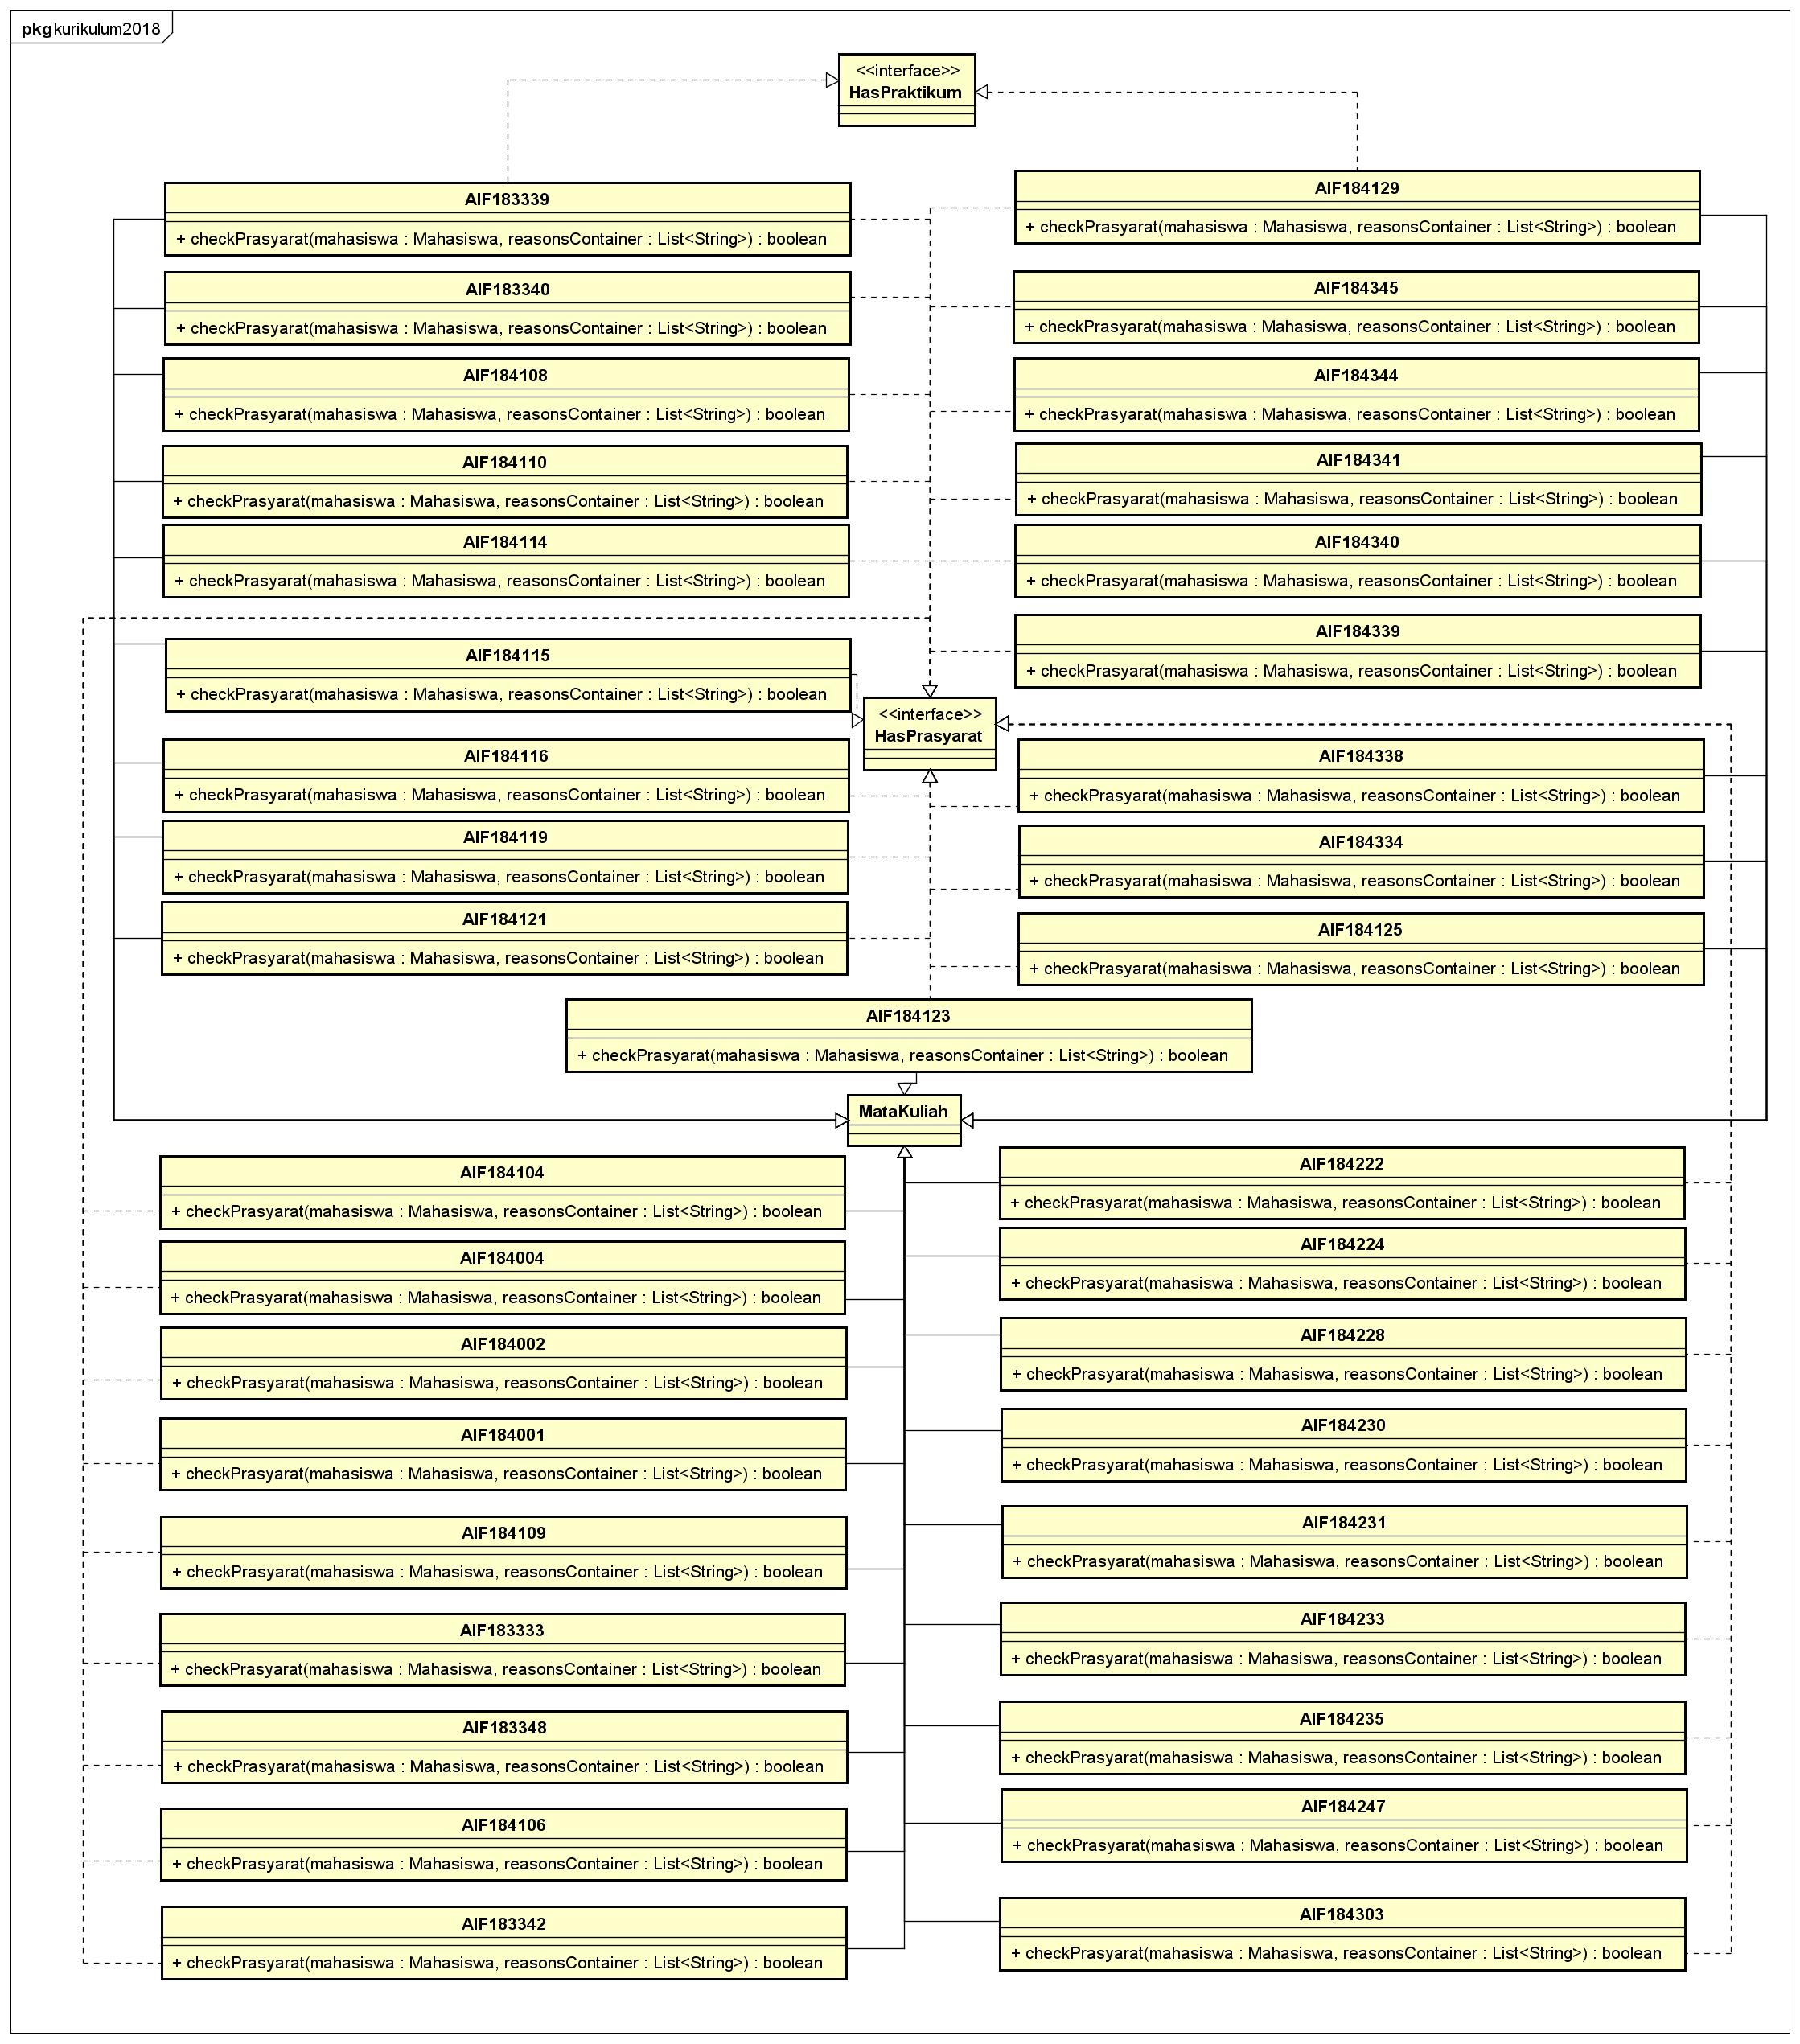
\includegraphics[scale=0.135]{Gambar/class-diagram-siamodels-mk-kurikulum-2018-5}
\caption{Diagram Kelas SIAModels \textit{Package} \texttt{kurikulum2018} 5}
\label{fig:siamodels_class_2018_kurikulum_5}
\end{figure}

\begin{enumerate}
	\item \textit{Package} \texttt{id.ac.unpar.siamodels.matakuliah.kurikulum2018} \\
	\textit{Package} ini berisi kelas-kelas yang merepresentasikan mata kuliah pada kurikulum 2018 berserta aturan prasyaratnya. Kelas-kelas yang ada pada \textit{package} ini adalah sebagai berikut:
	\begin{itemize}
		\item \texttt{AIF181091\_02} \\
		Kelas ini merepresentasikan mata kuliah Bahasa Inggris.
		\item \texttt{AIF181100\_04} \\
		Kelas ini merepresentasikan mata kuliah Dasar Pemrograman. Method yang dimiliki kelas ini adalah sebagai berikut: 
		\begin{itemize}
			\item \textbf{public boolean checkPrasyarat(Mahasiswa mahasiswa, List<String> reasonsContainer)}\\
			Memeriksa prasyarat-prasyarat dari kuliah, spesifik untuk mahasiswa yang dituju. Jika ada pesan-pesan khusus, akan ditambahkan pada parameter reasonsContainer.\\
			\textbf{Parameter:}
			\begin{itemize}
				\item \textbf{mahasiswa} prasyarat kuliah akan diperiksa spesifik pada mahasiswa ini.
				\item \textbf{reasonsContainer} jika pesan-pesan terkait prasyarat akan ditambahkan di sini.
			\end{itemize}
			\textbf{Kembalian:} \texttt{true} jika seluruh prasyarat dipenuhi, \texttt{false} jika tidak.
		\end{itemize}
		\item \texttt{AIF181101\_03} \\
		Kelas ini merepresentasikan mata kuliah Computational Thinking.
		\item \texttt{AIF181103\_04} \\
		Kelas ini merepresentasikan mata kuliah Matematika Dasar.
		\item \texttt{AIF181104\_03} \\
		Kelas ini merepresentasikan mata kuliah Logika Informatika.
		\item \texttt{AIF181105\_02} \\
		Kelas ini merepresentasikan mata kuliah Pengantar Informatika.
		\item \texttt{AIF181106\_03} \\
		Kelas ini merepresentasikan mata kuliah Matriks dan Ruang Vektor.
		\item \texttt{AIF181107\_03} \\
		Kelas ini merepresentasikan mata kuliah Matematika Diskret.
		\item \texttt{AIF181193\_03} \\
		Kelas ini merepresentasikan mata kuliah Matematika Dasar.
		\item \texttt{AIF181194\_02} \\
		Kelas ini merepresentasikan mata kuliah Logika Informatika.
		\item \texttt{AIF181195\_03} \\
		Kelas ini merepresentasikan mata kuliah Pengantar Informatika.
		\item \texttt{AIF181202\_04} \\
		Kelas ini merepresentasikan mata kuliah Arsitektur dan Organisasi Komputer.
		\item \texttt{AIF181298\_03} \\
		Kelas ini merepresentasikan mata kuliah Sistem Dijital.
		\item \texttt{AIF182007\_02} \\
		Kelas ini merepresentasikan mata kuliah Teknik Presentasi.
		\item \texttt{AIF182100\_04} \\
		Kelas ini merepresentasikan mata kuliah Analisis Desain Berorientasi Objek. Method yang dimiliki kelas ini adalah sebagai berikut: 
		\begin{itemize}
			\item \textbf{public boolean checkPrasyarat(Mahasiswa mahasiswa, List<String> reasonsContainer)}\\
			Memeriksa prasyarat-prasyarat dari kuliah, spesifik untuk mahasiswa yang dituju. Jika ada pesan-pesan khusus, akan ditambahkan pada parameter reasonsContainer.\\
			\textbf{Parameter:}
			\begin{itemize}
				\item \textbf{mahasiswa} prasyarat kuliah akan diperiksa spesifik pada mahasiswa ini.
				\item \textbf{reasonsContainer} jika pesan-pesan terkait prasyarat akan ditambahkan di sini.
			\end{itemize}
			\textbf{Kembalian:} \texttt{true} jika seluruh prasyarat dipenuhi, \texttt{false} jika tidak.
		\end{itemize}
		\item \texttt{AIF182101\_03} \\
		Kelas ini merepresentasikan mata kuliah Algoritma dan Struktur Data. Method yang dimiliki kelas ini adalah sebagai berikut: 
		\begin{itemize}
			\item \textbf{public boolean checkPrasyarat(Mahasiswa mahasiswa, List<String> reasonsContainer)}\\
			Memeriksa prasyarat-prasyarat dari kuliah, spesifik untuk mahasiswa yang dituju. Jika ada pesan-pesan khusus, akan ditambahkan pada parameter reasonsContainer.\\
			\textbf{Parameter:}
			\begin{itemize}
				\item \textbf{mahasiswa} prasyarat kuliah akan diperiksa spesifik pada mahasiswa ini.
				\item \textbf{reasonsContainer} jika pesan-pesan terkait prasyarat akan ditambahkan di sini.
			\end{itemize}
			\textbf{Kembalian:} \texttt{true} jika seluruh prasyarat dipenuhi, \texttt{false} jika tidak.
		\end{itemize}
		\item \texttt{AIF182103\_04} \\
		Kelas ini merepresentasikan mata kuliah Struktur Diskret. Method yang dimiliki kelas ini adalah sebagai berikut: 
		\begin{itemize}
			\item \textbf{public boolean checkPrasyarat(Mahasiswa mahasiswa, List<String> reasonsContainer)}\\
			Memeriksa prasyarat-prasyarat dari kuliah, spesifik untuk mahasiswa yang dituju. Jika ada pesan-pesan khusus, akan ditambahkan pada parameter reasonsContainer.\\
			\textbf{Parameter:}
			\begin{itemize}
				\item \textbf{mahasiswa} prasyarat kuliah akan diperiksa spesifik pada mahasiswa ini.
				\item \textbf{reasonsContainer} jika pesan-pesan terkait prasyarat akan ditambahkan di sini.
			\end{itemize}
			\textbf{Kembalian:} \texttt{true} jika seluruh prasyarat dipenuhi, \texttt{false} jika tidak.
		\end{itemize}
		\item \texttt{AIF182105\_02} \\
		Kelas ini merepresentasikan mata kuliah Pemrograman Berorientasi Objek. Method yang dimiliki kelas ini adalah sebagai berikut: 
		\begin{itemize}
			\item \textbf{public boolean checkPrasyarat(Mahasiswa mahasiswa, List<String> reasonsContainer)}\\
			Memeriksa prasyarat-prasyarat dari kuliah, spesifik untuk mahasiswa yang dituju. Jika ada pesan-pesan khusus, akan ditambahkan pada parameter reasonsContainer.\\
			\textbf{Parameter:}
			\begin{itemize}
				\item \textbf{mahasiswa} prasyarat kuliah akan diperiksa spesifik pada mahasiswa ini.
				\item \textbf{reasonsContainer} jika pesan-pesan terkait prasyarat akan ditambahkan di sini.
			\end{itemize}
			\textbf{Kembalian:} \texttt{true} jika seluruh prasyarat dipenuhi, \texttt{false} jika tidak.
		\end{itemize}
		\item \texttt{AIF182109\_03} \\
		Kelas ini merepresentasikan mata kuliah Statistika untuk Komputasi.
		\item \texttt{AIF182110\_02} \\
		Kelas ini merepresentasikan mata kuliah Pemrograman Fungsional. Method yang dimiliki kelas ini adalah sebagai berikut: 
		\begin{itemize}
			\item \textbf{public boolean checkPrasyarat(Mahasiswa mahasiswa, List<String> reasonsContainer)}\\
			Memeriksa prasyarat-prasyarat dari kuliah, spesifik untuk mahasiswa yang dituju. Jika ada pesan-pesan khusus, akan ditambahkan pada parameter reasonsContainer.\\
			\textbf{Parameter:}
			\begin{itemize}
				\item \textbf{mahasiswa} prasyarat kuliah akan diperiksa spesifik pada mahasiswa ini.
				\item \textbf{reasonsContainer} jika pesan-pesan terkait prasyarat akan ditambahkan di sini.
			\end{itemize}
			\textbf{Kembalian:} \texttt{true} jika seluruh prasyarat dipenuhi, \texttt{false} jika tidak.
		\end{itemize}
		\item \texttt{AIF182112\_03} \\
		Kelas ini merepresentasikan mata kuliah Pemodelan Formal. Method yang dimiliki kelas ini adalah sebagai berikut: 
		\begin{itemize}
			\item \textbf{public boolean checkPrasyarat(Mahasiswa mahasiswa, List<String> reasonsContainer)}\\
			Memeriksa prasyarat-prasyarat dari kuliah, spesifik untuk mahasiswa yang dituju. Jika ada pesan-pesan khusus, akan ditambahkan pada parameter reasonsContainer.\\
			\textbf{Parameter:}
			\begin{itemize}
				\item \textbf{mahasiswa} prasyarat kuliah akan diperiksa spesifik pada mahasiswa ini.
				\item \textbf{reasonsContainer} jika pesan-pesan terkait prasyarat akan ditambahkan di sini.
			\end{itemize}
			\textbf{Kembalian:} \texttt{true} jika seluruh prasyarat dipenuhi, \texttt{false} jika tidak.
		\end{itemize}
		\item \texttt{AIF182114\_03} \\
		Kelas ini merepresentasikan mata kuliah Pemrograman Kompetitif 1. Method yang dimiliki kelas ini adalah sebagai berikut: 
		\begin{itemize}
			\item \textbf{public boolean checkPrasyarat(Mahasiswa mahasiswa, List<String> reasonsContainer)}\\
			Memeriksa prasyarat-prasyarat dari kuliah, spesifik untuk mahasiswa yang dituju. Jika ada pesan-pesan khusus, akan ditambahkan pada parameter reasonsContainer.\\
			\textbf{Parameter:}
			\begin{itemize}
				\item \textbf{mahasiswa} prasyarat kuliah akan diperiksa spesifik pada mahasiswa ini.
				\item \textbf{reasonsContainer} jika pesan-pesan terkait prasyarat akan ditambahkan di sini.
			\end{itemize}
			\textbf{Kembalian:} \texttt{true} jika seluruh prasyarat dipenuhi, \texttt{false} jika tidak.
		\end{itemize}
		\item \texttt{AIF182116\_02} \\
		Kelas ini merepresentasikan mata kuliah Dasar-dasar Java. Method yang dimiliki kelas ini adalah sebagai berikut: 
		\begin{itemize}
			\item \textbf{public boolean checkPrasyarat(Mahasiswa mahasiswa, List<String> reasonsContainer)}\\
			Memeriksa prasyarat-prasyarat dari kuliah, spesifik untuk mahasiswa yang dituju. Jika ada pesan-pesan khusus, akan ditambahkan pada parameter reasonsContainer.\\
			\textbf{Parameter:}
			\begin{itemize}
				\item \textbf{mahasiswa} prasyarat kuliah akan diperiksa spesifik pada mahasiswa ini.
				\item \textbf{reasonsContainer} jika pesan-pesan terkait prasyarat akan ditambahkan di sini.
			\end{itemize}
			\textbf{Kembalian:} \texttt{true} jika seluruh prasyarat dipenuhi, \texttt{false} jika tidak.
		\end{itemize}
		\item \texttt{AIF182118\_03} \\
		Kelas ini merepresentasikan mata kuliah Teori Bilangan. Method yang dimiliki kelas ini adalah sebagai berikut: 
		\begin{itemize}
			\item \textbf{public boolean checkPrasyarat(Mahasiswa mahasiswa, List<String> reasonsContainer)}\\
			Memeriksa prasyarat-prasyarat dari kuliah, spesifik untuk mahasiswa yang dituju. Jika ada pesan-pesan khusus, akan ditambahkan pada parameter reasonsContainer.\\
			\textbf{Parameter:}
			\begin{itemize}
				\item \textbf{mahasiswa} prasyarat kuliah akan diperiksa spesifik pada mahasiswa ini.
				\item \textbf{reasonsContainer} jika pesan-pesan terkait prasyarat akan ditambahkan di sini.
			\end{itemize}
			\textbf{Kembalian:} \texttt{true} jika seluruh prasyarat dipenuhi, \texttt{false} jika tidak.
		\end{itemize}
		\item \texttt{AIF182120\_02} \\
		Kelas ini merepresentasikan mata kuliah Teori Bahasa dan Kompilasi. Method yang dimiliki kelas ini adalah sebagai berikut: 
		\begin{itemize}
			\item \textbf{public boolean checkPrasyarat(Mahasiswa mahasiswa, List<String> reasonsContainer)}\\
			Memeriksa prasyarat-prasyarat dari kuliah, spesifik untuk mahasiswa yang dituju. Jika ada pesan-pesan khusus, akan ditambahkan pada parameter reasonsContainer.\\
			\textbf{Parameter:}
			\begin{itemize}
				\item \textbf{mahasiswa} prasyarat kuliah akan diperiksa spesifik pada mahasiswa ini.
				\item \textbf{reasonsContainer} jika pesan-pesan terkait prasyarat akan ditambahkan di sini.
			\end{itemize}
			\textbf{Kembalian:} \texttt{true} jika seluruh prasyarat dipenuhi, \texttt{false} jika tidak.
		\end{itemize}
		\item \texttt{AIF182122\_03} \\
		Kelas ini merepresentasikan mata kuliah Matematika Kombinatorial. Method yang dimiliki kelas ini adalah sebagai berikut: 
		\begin{itemize}
			\item \textbf{public boolean checkPrasyarat(Mahasiswa mahasiswa, List<String> reasonsContainer)}\\
			Memeriksa prasyarat-prasyarat dari kuliah, spesifik untuk mahasiswa yang dituju. Jika ada pesan-pesan khusus, akan ditambahkan pada parameter reasonsContainer.\\
			\textbf{Parameter:}
			\begin{itemize}
				\item \textbf{mahasiswa} prasyarat kuliah akan diperiksa spesifik pada mahasiswa ini.
				\item \textbf{reasonsContainer} jika pesan-pesan terkait prasyarat akan ditambahkan di sini.
			\end{itemize}
			\textbf{Kembalian:} \texttt{true} jika seluruh prasyarat dipenuhi, \texttt{false} jika tidak.
		\end{itemize}
		\item \texttt{AIF182124\_03} \\
		Kelas ini merepresentasikan mata kuliah Metode Numerik. Method yang dimiliki kelas ini adalah sebagai berikut: 
		\begin{itemize}
			\item \textbf{public boolean checkPrasyarat(Mahasiswa mahasiswa, List<String> reasonsContainer)}\\
			Memeriksa prasyarat-prasyarat dari kuliah, spesifik untuk mahasiswa yang dituju. Jika ada pesan-pesan khusus, akan ditambahkan pada parameter reasonsContainer.\\
			\textbf{Parameter:}
			\begin{itemize}
				\item \textbf{mahasiswa} prasyarat kuliah akan diperiksa spesifik pada mahasiswa ini.
				\item \textbf{reasonsContainer} jika pesan-pesan terkait prasyarat akan ditambahkan di sini.
			\end{itemize}
			\textbf{Kembalian:} \texttt{true} jika seluruh prasyarat dipenuhi, \texttt{false} jika tidak.
		\end{itemize}
		\item \texttt{AIF182126\_02} \\
		Kelas ini merepresentasikan mata kuliah Pemrograman Lojik. Method yang dimiliki kelas ini adalah sebagai berikut: 
		\begin{itemize}
			\item \textbf{public boolean checkPrasyarat(Mahasiswa mahasiswa, List<String> reasonsContainer)}\\
			Memeriksa prasyarat-prasyarat dari kuliah, spesifik untuk mahasiswa yang dituju. Jika ada pesan-pesan khusus, akan ditambahkan pada parameter reasonsContainer.\\
			\textbf{Parameter:}
			\begin{itemize}
				\item \textbf{mahasiswa} prasyarat kuliah akan diperiksa spesifik pada mahasiswa ini.
				\item \textbf{reasonsContainer} jika pesan-pesan terkait prasyarat akan ditambahkan di sini.
			\end{itemize}
			\textbf{Kembalian:} \texttt{true} jika seluruh prasyarat dipenuhi, \texttt{false} jika tidak.
		\end{itemize}
		\item \texttt{AIF182190\_03} \\
		Kelas ini merepresentasikan mata kuliah Analisis Desain Berorientasi  Objek.
		\item \texttt{AIF182191\_01} \\
		Kelas ini merepresentasikan mata kuliah Praktika Algoritma dan Struktur Data.
		\item \texttt{AIF182195\_01} \\
		Kelas ini merepresentasikan mata kuliah Praktika Pemrograman Berorientasi Objek.
		\item \texttt{AIF182204\_03} \\
		Kelas ini merepresentasikan mata kuliah Pemrograman Berbasis Web. Method yang dimiliki kelas ini adalah sebagai berikut: 
		\begin{itemize}
			\item \textbf{public boolean checkPrasyarat(Mahasiswa mahasiswa, List<String> reasonsContainer)}\\
			Memeriksa prasyarat-prasyarat dari kuliah, spesifik untuk mahasiswa yang dituju. Jika ada pesan-pesan khusus, akan ditambahkan pada parameter reasonsContainer.\\
			\textbf{Parameter:}
			\begin{itemize}
				\item \textbf{mahasiswa} prasyarat kuliah akan diperiksa spesifik pada mahasiswa ini.
				\item \textbf{reasonsContainer} jika pesan-pesan terkait prasyarat akan ditambahkan di sini.
			\end{itemize}
			\textbf{Kembalian:} \texttt{true} jika seluruh prasyarat dipenuhi, \texttt{false} jika tidak.
		\end{itemize}
		\item \texttt{AIF182206\_03} \\
		Kelas ini merepresentasikan mata kuliah Sistem Operasi. Method yang dimiliki kelas ini adalah sebagai berikut: 
		\begin{itemize}
			\item \textbf{public boolean checkPrasyarat(Mahasiswa mahasiswa, List<String> reasonsContainer)}\\
			Memeriksa prasyarat-prasyarat dari kuliah, spesifik untuk mahasiswa yang dituju. Jika ada pesan-pesan khusus, akan ditambahkan pada parameter reasonsContainer.\\
			\textbf{Parameter:}
			\begin{itemize}
				\item \textbf{mahasiswa} prasyarat kuliah akan diperiksa spesifik pada mahasiswa ini.
				\item \textbf{reasonsContainer} jika pesan-pesan terkait prasyarat akan ditambahkan di sini.
			\end{itemize}
			\textbf{Kembalian:} \texttt{true} jika seluruh prasyarat dipenuhi, \texttt{false} jika tidak.
		\end{itemize}
		\item \texttt{AIF182294\_02} \\
		Kelas ini merepresentasikan mata kuliah Pemrograman Berbasis Web.
		\item \texttt{AIF182296\_01} \\
		Kelas ini merepresentasikan mata kuliah Praktika Sistem Operasi.
		\item \texttt{AIF182302\_04} \\
		Kelas ini merepresentasikan mata kuliah Majemen Informasi dan Basis Data. Method yang dimiliki kelas ini adalah sebagai berikut: 
		\begin{itemize}
			\item \textbf{public boolean checkPrasyarat(Mahasiswa mahasiswa, List<String> reasonsContainer)}\\
			Memeriksa prasyarat-prasyarat dari kuliah, spesifik untuk mahasiswa yang dituju. Jika ada pesan-pesan khusus, akan ditambahkan pada parameter reasonsContainer.\\
			\textbf{Parameter:}
			\begin{itemize}
				\item \textbf{mahasiswa} prasyarat kuliah akan diperiksa spesifik pada mahasiswa ini.
				\item \textbf{reasonsContainer} jika pesan-pesan terkait prasyarat akan ditambahkan di sini.
			\end{itemize}
			\textbf{Kembalian:} \texttt{true} jika seluruh prasyarat dipenuhi, \texttt{false} jika tidak.
		\end{itemize}
		\item \texttt{AIF182308\_03} \\
		Kelas ini merepresentasikan mata kuliah Pengantar Sistem Informasi. Method yang dimiliki kelas ini adalah sebagai berikut: 
		\begin{itemize}
			\item \textbf{public boolean checkPrasyarat(Mahasiswa mahasiswa, List<String> reasonsContainer)}\\
			Memeriksa prasyarat-prasyarat dari kuliah, spesifik untuk mahasiswa yang dituju. Jika ada pesan-pesan khusus, akan ditambahkan pada parameter reasonsContainer.\\
			\textbf{Parameter:}
			\begin{itemize}
				\item \textbf{mahasiswa} prasyarat kuliah akan diperiksa spesifik pada mahasiswa ini.
				\item \textbf{reasonsContainer} jika pesan-pesan terkait prasyarat akan ditambahkan di sini.
			\end{itemize}
			\textbf{Kembalian:} \texttt{true} jika seluruh prasyarat dipenuhi, \texttt{false} jika tidak.
		\end{itemize}
		\item \texttt{AIF182392\_03} \\
		Kelas ini merepresentasikan mata kuliah Manajemen Informasi dan Basis Data.
		\item \texttt{AIF183002\_02} \\
		Kelas ini merepresentasikan mata kuliah Penulisan Ilmiah.
		\item \texttt{AIF183010\_03} \\
		Kelas ini merepresentasikan mata kuliah Kerja Praktek 2.
		\item \texttt{AIF183013\_02} \\
		Kelas ini merepresentasikan mata kuliah Kerja Praktek 1.
		\item \texttt{AIF183015\_03} \\
		Kelas ini merepresentasikan mata kuliah Pendidikan Pengabdian kepada Masyarakat.
		\item \texttt{AIF183100\_03} \\
		Kelas ini merepresentasikan mata kuliah Pengantar Sistem Cerdas. Method yang dimiliki kelas ini adalah sebagai berikut: 
		\begin{itemize}
			\item \textbf{public boolean checkPrasyarat(Mahasiswa mahasiswa, List<String> reasonsContainer)}\\
			Memeriksa prasyarat-prasyarat dari kuliah, spesifik untuk mahasiswa yang dituju. Jika ada pesan-pesan khusus, akan ditambahkan pada parameter reasonsContainer.\\
			\textbf{Parameter:}
			\begin{itemize}
				\item \textbf{mahasiswa} prasyarat kuliah akan diperiksa spesifik pada mahasiswa ini.
				\item \textbf{reasonsContainer} jika pesan-pesan terkait prasyarat akan ditambahkan di sini.
			\end{itemize}
			\textbf{Kembalian:} \texttt{true} jika seluruh prasyarat dipenuhi, \texttt{false} jika tidak.
		\end{itemize}
		\item \texttt{AIF183101\_03} \\
		Kelas ini merepresentasikan mata kuliah Desain dan Analisis Algoritma. Method yang dimiliki kelas ini adalah sebagai berikut: 
		\begin{itemize}
			\item \textbf{public boolean checkPrasyarat(Mahasiswa mahasiswa, List<String> reasonsContainer)}\\
			Memeriksa prasyarat-prasyarat dari kuliah, spesifik untuk mahasiswa yang dituju. Jika ada pesan-pesan khusus, akan ditambahkan pada parameter reasonsContainer.\\
			\textbf{Parameter:}
			\begin{itemize}
				\item \textbf{mahasiswa} prasyarat kuliah akan diperiksa spesifik pada mahasiswa ini.
				\item \textbf{reasonsContainer} jika pesan-pesan terkait prasyarat akan ditambahkan di sini.
			\end{itemize}
			\textbf{Kembalian:} \texttt{true} jika seluruh prasyarat dipenuhi, \texttt{false} jika tidak.
		\end{itemize}
		\item \texttt{AIF183104\_03} \\
		Kelas ini merepresentasikan mata kuliah Interaksi Manusia Komputer.
		\item \texttt{AIF183106\_06} \\
		Kelas ini merepresentasikan mata kuliah Proyek Informatika. Method yang dimiliki kelas ini adalah sebagai berikut: 
		\begin{itemize}
			\item \textbf{public boolean checkPrasyarat(Mahasiswa mahasiswa, List<String> reasonsContainer)}\\
			Memeriksa prasyarat-prasyarat dari kuliah, spesifik untuk mahasiswa yang dituju. Jika ada pesan-pesan khusus, akan ditambahkan pada parameter reasonsContainer.\\
			\textbf{Parameter:}
			\begin{itemize}
				\item \textbf{mahasiswa} prasyarat kuliah akan diperiksa spesifik pada mahasiswa ini.
				\item \textbf{reasonsContainer} jika pesan-pesan terkait prasyarat akan ditambahkan di sini.
			\end{itemize}
			\textbf{Kembalian:} \texttt{true} jika seluruh prasyarat dipenuhi, \texttt{false} jika tidak.
		\end{itemize}
		\item \texttt{AIF183112\_02} \\
		Kelas ini merepresentasikan mata kuliah Pengujian Perangkat Lunak. Method yang dimiliki kelas ini adalah sebagai berikut: 
		\begin{itemize}
			\item \textbf{public boolean checkPrasyarat(Mahasiswa mahasiswa, List<String> reasonsContainer)}\\
			Memeriksa prasyarat-prasyarat dari kuliah, spesifik untuk mahasiswa yang dituju. Jika ada pesan-pesan khusus, akan ditambahkan pada parameter reasonsContainer.\\
			\textbf{Parameter:}
			\begin{itemize}
				\item \textbf{mahasiswa} prasyarat kuliah akan diperiksa spesifik pada mahasiswa ini.
				\item \textbf{reasonsContainer} jika pesan-pesan terkait prasyarat akan ditambahkan di sini.
			\end{itemize}
			\textbf{Kembalian:} \texttt{true} jika seluruh prasyarat dipenuhi, \texttt{false} jika tidak.
		\end{itemize}
		\item \texttt{AIF183114\_03} \\
		Kelas ini merepresentasikan mata kuliah Algoritma Kriptografi. Method yang dimiliki kelas ini adalah sebagai berikut: 
		\begin{itemize}
			\item \textbf{public boolean checkPrasyarat(Mahasiswa mahasiswa, List<String> reasonsContainer)}\\
			Memeriksa prasyarat-prasyarat dari kuliah, spesifik untuk mahasiswa yang dituju. Jika ada pesan-pesan khusus, akan ditambahkan pada parameter reasonsContainer.\\
			\textbf{Parameter:}
			\begin{itemize}
				\item \textbf{mahasiswa} prasyarat kuliah akan diperiksa spesifik pada mahasiswa ini.
				\item \textbf{reasonsContainer} jika pesan-pesan terkait prasyarat akan ditambahkan di sini.
			\end{itemize}
			\textbf{Kembalian:} \texttt{true} jika seluruh prasyarat dipenuhi, \texttt{false} jika tidak.
		\end{itemize}
		\item \texttt{AIF183116\_02} \\
		Kelas ini merepresentasikan mata kuliah Komputasi Paralel. Method yang dimiliki kelas ini adalah sebagai berikut: 
		\begin{itemize}
			\item \textbf{public boolean checkPrasyarat(Mahasiswa mahasiswa, List<String> reasonsContainer)}\\
			Memeriksa prasyarat-prasyarat dari kuliah, spesifik untuk mahasiswa yang dituju. Jika ada pesan-pesan khusus, akan ditambahkan pada parameter reasonsContainer.\\
			\textbf{Parameter:}
			\begin{itemize}
				\item \textbf{mahasiswa} prasyarat kuliah akan diperiksa spesifik pada mahasiswa ini.
				\item \textbf{reasonsContainer} jika pesan-pesan terkait prasyarat akan ditambahkan di sini.
			\end{itemize}
			\textbf{Kembalian:} \texttt{true} jika seluruh prasyarat dipenuhi, \texttt{false} jika tidak.
		\end{itemize}
		\item \texttt{AIF183117\_02} \\
		Kelas ini merepresentasikan mata kuliah Grafika Komputer. Method yang dimiliki kelas ini adalah sebagai berikut: 
		\begin{itemize}
			\item \textbf{public boolean checkPrasyarat(Mahasiswa mahasiswa, List<String> reasonsContainer)}\\
			Memeriksa prasyarat-prasyarat dari kuliah, spesifik untuk mahasiswa yang dituju. Jika ada pesan-pesan khusus, akan ditambahkan pada parameter reasonsContainer.\\
			\textbf{Parameter:}
			\begin{itemize}
				\item \textbf{mahasiswa} prasyarat kuliah akan diperiksa spesifik pada mahasiswa ini.
				\item \textbf{reasonsContainer} jika pesan-pesan terkait prasyarat akan ditambahkan di sini.
			\end{itemize}
			\textbf{Kembalian:} \texttt{true} jika seluruh prasyarat dipenuhi, \texttt{false} jika tidak.
		\end{itemize}
		\item \texttt{AIF183118\_03} \\
		Kelas ini merepresentasikan mata kuliah Komputasi Geometri. Method yang dimiliki kelas ini adalah sebagai berikut: 
		\begin{itemize}
			\item \textbf{public boolean checkPrasyarat(Mahasiswa mahasiswa, List<String> reasonsContainer)}\\
			Memeriksa prasyarat-prasyarat dari kuliah, spesifik untuk mahasiswa yang dituju. Jika ada pesan-pesan khusus, akan ditambahkan pada parameter reasonsContainer.\\
			\textbf{Parameter:}
			\begin{itemize}
				\item \textbf{mahasiswa} prasyarat kuliah akan diperiksa spesifik pada mahasiswa ini.
				\item \textbf{reasonsContainer} jika pesan-pesan terkait prasyarat akan ditambahkan di sini.
			\end{itemize}
			\textbf{Kembalian:} \texttt{true} jika seluruh prasyarat dipenuhi, \texttt{false} jika tidak.
		\end{itemize}
		\item \texttt{AIF183119\_02} \\
		Kelas ini merepresentasikan mata kuliah Keamanan Informasi. Method yang dimiliki kelas ini adalah sebagai berikut: 
		\begin{itemize}
			\item \textbf{public boolean checkPrasyarat(Mahasiswa mahasiswa, List<String> reasonsContainer)}\\
			Memeriksa prasyarat-prasyarat dari kuliah, spesifik untuk mahasiswa yang dituju. Jika ada pesan-pesan khusus, akan ditambahkan pada parameter reasonsContainer.\\
			\textbf{Parameter:}
			\begin{itemize}
				\item \textbf{mahasiswa} prasyarat kuliah akan diperiksa spesifik pada mahasiswa ini.
				\item \textbf{reasonsContainer} jika pesan-pesan terkait prasyarat akan ditambahkan di sini.
			\end{itemize}
			\textbf{Kembalian:} \texttt{true} jika seluruh prasyarat dipenuhi, \texttt{false} jika tidak.
		\end{itemize}
		\item \texttt{AIF183120\_03} \\
		Kelas ini merepresentasikan mata kuliah Perancangan Permainan Komputer. Method yang dimiliki kelas ini adalah sebagai berikut: 
		\begin{itemize}
			\item \textbf{public boolean checkPrasyarat(Mahasiswa mahasiswa, List<String> reasonsContainer)}\\
			Memeriksa prasyarat-prasyarat dari kuliah, spesifik untuk mahasiswa yang dituju. Jika ada pesan-pesan khusus, akan ditambahkan pada parameter reasonsContainer.\\
			\textbf{Parameter:}
			\begin{itemize}
				\item \textbf{mahasiswa} prasyarat kuliah akan diperiksa spesifik pada mahasiswa ini.
				\item \textbf{reasonsContainer} jika pesan-pesan terkait prasyarat akan ditambahkan di sini.
			\end{itemize}
			\textbf{Kembalian:} \texttt{true} jika seluruh prasyarat dipenuhi, \texttt{false} jika tidak.
		\end{itemize}
		\item \texttt{AIF183121\_03} \\
		Kelas ini merepresentasikan mata kuliah Pemrograman Kompetitif 2. Method yang dimiliki kelas ini adalah sebagai berikut: 
		\begin{itemize}
			\item \textbf{public boolean checkPrasyarat(Mahasiswa mahasiswa, List<String> reasonsContainer)}\\
			Memeriksa prasyarat-prasyarat dari kuliah, spesifik untuk mahasiswa yang dituju. Jika ada pesan-pesan khusus, akan ditambahkan pada parameter reasonsContainer.\\
			\textbf{Parameter:}
			\begin{itemize}
				\item \textbf{mahasiswa} prasyarat kuliah akan diperiksa spesifik pada mahasiswa ini.
				\item \textbf{reasonsContainer} jika pesan-pesan terkait prasyarat akan ditambahkan di sini.
			\end{itemize}
			\textbf{Kembalian:} \texttt{true} jika seluruh prasyarat dipenuhi, \texttt{false} jika tidak.
		\end{itemize}
		\item \texttt{AIF183122\_03} \\
		Kelas ini merepresentasikan mata kuliah Pemodelan Simulasi. Method yang dimiliki kelas ini adalah sebagai berikut: 
		\begin{itemize}
			\item \textbf{public boolean checkPrasyarat(Mahasiswa mahasiswa, List<String> reasonsContainer)}\\
			Memeriksa prasyarat-prasyarat dari kuliah, spesifik untuk mahasiswa yang dituju. Jika ada pesan-pesan khusus, akan ditambahkan pada parameter reasonsContainer.\\
			\textbf{Parameter:}
			\begin{itemize}
				\item \textbf{mahasiswa} prasyarat kuliah akan diperiksa spesifik pada mahasiswa ini.
				\item \textbf{reasonsContainer} jika pesan-pesan terkait prasyarat akan ditambahkan di sini.
			\end{itemize}
			\textbf{Kembalian:} \texttt{true} jika seluruh prasyarat dipenuhi, \texttt{false} jika tidak.
		\end{itemize}
		\item \texttt{AIF183123\_02} \\
		Kelas ini merepresentasikan mata kuliah Topik Khusus Informatika 1.
		\item \texttt{AIF183124\_03} \\
		Kelas ini merepresentasikan mata kuliah Grafika Komputer Lanjut. Method yang dimiliki kelas ini adalah sebagai berikut: 
		\begin{itemize}
			\item \textbf{public boolean checkPrasyarat(Mahasiswa mahasiswa, List<String> reasonsContainer)}\\
			Memeriksa prasyarat-prasyarat dari kuliah, spesifik untuk mahasiswa yang dituju. Jika ada pesan-pesan khusus, akan ditambahkan pada parameter reasonsContainer.\\
			\textbf{Parameter:}
			\begin{itemize}
				\item \textbf{mahasiswa} prasyarat kuliah akan diperiksa spesifik pada mahasiswa ini.
				\item \textbf{reasonsContainer} jika pesan-pesan terkait prasyarat akan ditambahkan di sini.
			\end{itemize}
			\textbf{Kembalian:} \texttt{true} jika seluruh prasyarat dipenuhi, \texttt{false} jika tidak.
		\end{itemize}
		\item \texttt{AIF183126\_03} \\
		Kelas ini merepresentasikan mata kuliah Pemrograman Kompetitif 3. Method yang dimiliki kelas ini adalah sebagai berikut: 
		\begin{itemize}
			\item \textbf{public boolean checkPrasyarat(Mahasiswa mahasiswa, List<String> reasonsContainer)}\\
			Memeriksa prasyarat-prasyarat dari kuliah, spesifik untuk mahasiswa yang dituju. Jika ada pesan-pesan khusus, akan ditambahkan pada parameter reasonsContainer.\\
			\textbf{Parameter:}
			\begin{itemize}
				\item \textbf{mahasiswa} prasyarat kuliah akan diperiksa spesifik pada mahasiswa ini.
				\item \textbf{reasonsContainer} jika pesan-pesan terkait prasyarat akan ditambahkan di sini.
			\end{itemize}
			\textbf{Kembalian:} \texttt{true} jika seluruh prasyarat dipenuhi, \texttt{false} jika tidak.
		\end{itemize}
		\item \texttt{AIF183128\_03} \\
		Kelas ini merepresentasikan mata kuliah Topik Khusus Informatika 2.
		\item \texttt{AIF183191\_01} \\
		Kelas ini merepresentasikan mata kuliah Praktika Desain dan Analisis Algoritma .
		\item \texttt{AIF183194\_02} \\
		Kelas ini merepresentasikan mata kuliah Interaksi Manusia Komputer.
		\item \texttt{AIF183195\_02} \\
		Kelas ini merepresentasikan mata kuliah Desain Antarmuka Grafis.
		\item \texttt{AIF183197\_03} \\
		Kelas ini merepresentasikan mata kuliah Matematika Teknik.
		\item \texttt{AIF183209\_03} \\
		Kelas ini merepresentasikan mata kuliah Pemrograman Aplikasi Bergerak. Method yang dimiliki kelas ini adalah sebagai berikut: 
		\begin{itemize}
			\item \textbf{public boolean checkPrasyarat(Mahasiswa mahasiswa, List<String> reasonsContainer)}\\
			Memeriksa prasyarat-prasyarat dari kuliah, spesifik untuk mahasiswa yang dituju. Jika ada pesan-pesan khusus, akan ditambahkan pada parameter reasonsContainer.\\
			\textbf{Parameter:}
			\begin{itemize}
				\item \textbf{mahasiswa} prasyarat kuliah akan diperiksa spesifik pada mahasiswa ini.
				\item \textbf{reasonsContainer} jika pesan-pesan terkait prasyarat akan ditambahkan di sini.
			\end{itemize}
			\textbf{Kembalian:} \texttt{true} jika seluruh prasyarat dipenuhi, \texttt{false} jika tidak.
		\end{itemize}
		\item \texttt{AIF183211\_04} \\
		Kelas ini merepresentasikan mata kuliah Jaringan Komputer. Method yang dimiliki kelas ini adalah sebagai berikut: 
		\begin{itemize}
			\item \textbf{public boolean checkPrasyarat(Mahasiswa mahasiswa, List<String> reasonsContainer)}\\
			Memeriksa prasyarat-prasyarat dari kuliah, spesifik untuk mahasiswa yang dituju. Jika ada pesan-pesan khusus, akan ditambahkan pada parameter reasonsContainer.\\
			\textbf{Parameter:}
			\begin{itemize}
				\item \textbf{mahasiswa} prasyarat kuliah akan diperiksa spesifik pada mahasiswa ini.
				\item \textbf{reasonsContainer} jika pesan-pesan terkait prasyarat akan ditambahkan di sini.
			\end{itemize}
			\textbf{Kembalian:} \texttt{true} jika seluruh prasyarat dipenuhi, \texttt{false} jika tidak.
		\end{itemize}
		\item \texttt{AIF183225\_03} \\
		Kelas ini merepresentasikan mata kuliah Administrasi Jaringan Komputer 1.
		\item \texttt{AIF183227\_03} \\
		Kelas ini merepresentasikan mata kuliah Pengantar Telekomunikasi. Method yang dimiliki kelas ini adalah sebagai berikut: 
		\begin{itemize}
			\item \textbf{public boolean checkPrasyarat(Mahasiswa mahasiswa, List<String> reasonsContainer)}\\
			Memeriksa prasyarat-prasyarat dari kuliah, spesifik untuk mahasiswa yang dituju. Jika ada pesan-pesan khusus, akan ditambahkan pada parameter reasonsContainer.\\
			\textbf{Parameter:}
			\begin{itemize}
				\item \textbf{mahasiswa} prasyarat kuliah akan diperiksa spesifik pada mahasiswa ini.
				\item \textbf{reasonsContainer} jika pesan-pesan terkait prasyarat akan ditambahkan di sini.
			\end{itemize}
			\textbf{Kembalian:} \texttt{true} jika seluruh prasyarat dipenuhi, \texttt{false} jika tidak.
		\end{itemize}
		\item \texttt{AIF183229\_02} \\
		Kelas ini merepresentasikan mata kuliah Topik Khusus Sistem Terdistribusi 1.
		\item \texttt{AIF183230\_03} \\
		Kelas ini merepresentasikan mata kuliah Jaringan Komputer Lanjut. Method yang dimiliki kelas ini adalah sebagai berikut: 
		\begin{itemize}
			\item \textbf{public boolean checkPrasyarat(Mahasiswa mahasiswa, List<String> reasonsContainer)}\\
			Memeriksa prasyarat-prasyarat dari kuliah, spesifik untuk mahasiswa yang dituju. Jika ada pesan-pesan khusus, akan ditambahkan pada parameter reasonsContainer.\\
			\textbf{Parameter:}
			\begin{itemize}
				\item \textbf{mahasiswa} prasyarat kuliah akan diperiksa spesifik pada mahasiswa ini.
				\item \textbf{reasonsContainer} jika pesan-pesan terkait prasyarat akan ditambahkan di sini.
			\end{itemize}
			\textbf{Kembalian:} \texttt{true} jika seluruh prasyarat dipenuhi, \texttt{false} jika tidak.
		\end{itemize}
		\item \texttt{AIF183232\_03} \\
		Kelas ini merepresentasikan mata kuliah Pemrograman Berbasis Web Lanjut. Method yang dimiliki kelas ini adalah sebagai berikut: 
		\begin{itemize}
			\item \textbf{public boolean checkPrasyarat(Mahasiswa mahasiswa, List<String> reasonsContainer)}\\
			Memeriksa prasyarat-prasyarat dari kuliah, spesifik untuk mahasiswa yang dituju. Jika ada pesan-pesan khusus, akan ditambahkan pada parameter reasonsContainer.\\
			\textbf{Parameter:}
			\begin{itemize}
				\item \textbf{mahasiswa} prasyarat kuliah akan diperiksa spesifik pada mahasiswa ini.
				\item \textbf{reasonsContainer} jika pesan-pesan terkait prasyarat akan ditambahkan di sini.
			\end{itemize}
			\textbf{Kembalian:} \texttt{true} jika seluruh prasyarat dipenuhi, \texttt{false} jika tidak.
		\end{itemize}
		\item \texttt{AIF183234\_03} \\
		Kelas ini merepresentasikan mata kuliah Sistem Aplikasi Telematika. Method yang dimiliki kelas ini adalah sebagai berikut: 
		\begin{itemize}
			\item \textbf{public boolean checkPrasyarat(Mahasiswa mahasiswa, List<String> reasonsContainer)}\\
			Memeriksa prasyarat-prasyarat dari kuliah, spesifik untuk mahasiswa yang dituju. Jika ada pesan-pesan khusus, akan ditambahkan pada parameter reasonsContainer.\\
			\textbf{Parameter:}
			\begin{itemize}
				\item \textbf{mahasiswa} prasyarat kuliah akan diperiksa spesifik pada mahasiswa ini.
				\item \textbf{reasonsContainer} jika pesan-pesan terkait prasyarat akan ditambahkan di sini.
			\end{itemize}
			\textbf{Kembalian:} \texttt{true} jika seluruh prasyarat dipenuhi, \texttt{false} jika tidak.
		\end{itemize}
		\item \texttt{AIF183236\_03} \\
		Kelas ini merepresentasikan mata kuliah Administrasi Jaringan Komputer 2. Method yang dimiliki kelas ini adalah sebagai berikut: 
		\begin{itemize}
			\item \textbf{public boolean checkPrasyarat(Mahasiswa mahasiswa, List<String> reasonsContainer)}\\
			Memeriksa prasyarat-prasyarat dari kuliah, spesifik untuk mahasiswa yang dituju. Jika ada pesan-pesan khusus, akan ditambahkan pada parameter reasonsContainer.\\
			\textbf{Parameter:}
			\begin{itemize}
				\item \textbf{mahasiswa} prasyarat kuliah akan diperiksa spesifik pada mahasiswa ini.
				\item \textbf{reasonsContainer} jika pesan-pesan terkait prasyarat akan ditambahkan di sini.
			\end{itemize}
			\textbf{Kembalian:} \texttt{true} jika seluruh prasyarat dipenuhi, \texttt{false} jika tidak.
		\end{itemize}
		\item \texttt{AIF183238\_03} \\
		Kelas ini merepresentasikan mata kuliah Topik Khusus Sistem Terdistribusi 2.
		\item \texttt{AIF183290\_02} \\
		Kelas ini merepresentasikan mata kuliah Analisis Proses Bisnis.
		\item \texttt{AIF183299\_02} \\
		Kelas ini merepresentasikan mata kuliah Pemrograman Aplikasi Bergerak.
		\item \texttt{AIF183303\_03} \\
		Kelas ini merepresentasikan mata kuliah Rekayasa Perangkat Lunak. Method yang dimiliki kelas ini adalah sebagai berikut: 
		\begin{itemize}
			\item \textbf{public boolean checkPrasyarat(Mahasiswa mahasiswa, List<String> reasonsContainer)}\\
			Memeriksa prasyarat-prasyarat dari kuliah, spesifik untuk mahasiswa yang dituju. Jika ada pesan-pesan khusus, akan ditambahkan pada parameter reasonsContainer.\\
			\textbf{Parameter:}
			\begin{itemize}
				\item \textbf{mahasiswa} prasyarat kuliah akan diperiksa spesifik pada mahasiswa ini.
				\item \textbf{reasonsContainer} jika pesan-pesan terkait prasyarat akan ditambahkan di sini.
			\end{itemize}
			\textbf{Kembalian:} \texttt{true} jika seluruh prasyarat dipenuhi, \texttt{false} jika tidak.
		\end{itemize}
		\item \texttt{AIF183305\_02} \\
		Kelas ini merepresentasikan mata kuliah Manajemen Proyek. Method yang dimiliki kelas ini adalah sebagai berikut: 
		\begin{itemize}
			\item \textbf{public boolean checkPrasyarat(Mahasiswa mahasiswa, List<String> reasonsContainer)}\\
			Memeriksa prasyarat-prasyarat dari kuliah, spesifik untuk mahasiswa yang dituju. Jika ada pesan-pesan khusus, akan ditambahkan pada parameter reasonsContainer.\\
			\textbf{Parameter:}
			\begin{itemize}
				\item \textbf{mahasiswa} prasyarat kuliah akan diperiksa spesifik pada mahasiswa ini.
				\item \textbf{reasonsContainer} jika pesan-pesan terkait prasyarat akan ditambahkan di sini.
			\end{itemize}
			\textbf{Kembalian:} \texttt{true} jika seluruh prasyarat dipenuhi, \texttt{false} jika tidak.
		\end{itemize}
		\item \texttt{AIF183307\_02} \\
		Kelas ini merepresentasikan mata kuliah Teknologi Basis Data. Method yang dimiliki kelas ini adalah sebagai berikut: 
		\begin{itemize}
			\item \textbf{public boolean checkPrasyarat(Mahasiswa mahasiswa, List<String> reasonsContainer)}\\
			Memeriksa prasyarat-prasyarat dari kuliah, spesifik untuk mahasiswa yang dituju. Jika ada pesan-pesan khusus, akan ditambahkan pada parameter reasonsContainer.\\
			\textbf{Parameter:}
			\begin{itemize}
				\item \textbf{mahasiswa} prasyarat kuliah akan diperiksa spesifik pada mahasiswa ini.
				\item \textbf{reasonsContainer} jika pesan-pesan terkait prasyarat akan ditambahkan di sini.
			\end{itemize}
			\textbf{Kembalian:} \texttt{true} jika seluruh prasyarat dipenuhi, \texttt{false} jika tidak.
		\end{itemize}
		\item \texttt{AIF183308\_03} \\
		Kelas ini merepresentasikan mata kuliah Proyek Sistem Informasi 1. Method yang dimiliki kelas ini adalah sebagai berikut: 
		\begin{itemize}
			\item \textbf{public boolean checkPrasyarat(Mahasiswa mahasiswa, List<String> reasonsContainer)}\\
			Memeriksa prasyarat-prasyarat dari kuliah, spesifik untuk mahasiswa yang dituju. Jika ada pesan-pesan khusus, akan ditambahkan pada parameter reasonsContainer.\\
			\textbf{Parameter:}
			\begin{itemize}
				\item \textbf{mahasiswa} prasyarat kuliah akan diperiksa spesifik pada mahasiswa ini.
				\item \textbf{reasonsContainer} jika pesan-pesan terkait prasyarat akan ditambahkan di sini.
			\end{itemize}
			\textbf{Kembalian:} \texttt{true} jika seluruh prasyarat dipenuhi, \texttt{false} jika tidak.
		\end{itemize}
		\item \texttt{AIF183331\_03} \\
		Kelas ini merepresentasikan mata kuliah Sistem e-Commerce. Method yang dimiliki kelas ini adalah sebagai berikut: 
		\begin{itemize}
			\item \textbf{public boolean checkPrasyarat(Mahasiswa mahasiswa, List<String> reasonsContainer)}\\
			Memeriksa prasyarat-prasyarat dari kuliah, spesifik untuk mahasiswa yang dituju. Jika ada pesan-pesan khusus, akan ditambahkan pada parameter reasonsContainer.\\
			\textbf{Parameter:}
			\begin{itemize}
				\item \textbf{mahasiswa} prasyarat kuliah akan diperiksa spesifik pada mahasiswa ini.
				\item \textbf{reasonsContainer} jika pesan-pesan terkait prasyarat akan ditambahkan di sini.
			\end{itemize}
			\textbf{Kembalian:} \texttt{true} jika seluruh prasyarat dipenuhi, \texttt{false} jika tidak.
		\end{itemize}
		\item \texttt{AIF183333\_02} \\
		Kelas ini merepresentasikan mata kuliah Metodologi Pengembangan Sistem Informasi 1. Method yang dimiliki kelas ini adalah sebagai berikut: 
		\begin{itemize}
			\item \textbf{public boolean checkPrasyarat(Mahasiswa mahasiswa, List<String> reasonsContainer)}\\
			Memeriksa prasyarat-prasyarat dari kuliah, spesifik untuk mahasiswa yang dituju. Jika ada pesan-pesan khusus, akan ditambahkan pada parameter reasonsContainer.\\
			\textbf{Parameter:}
			\begin{itemize}
				\item \textbf{mahasiswa} prasyarat kuliah akan diperiksa spesifik pada mahasiswa ini.
				\item \textbf{reasonsContainer} jika pesan-pesan terkait prasyarat akan ditambahkan di sini.
			\end{itemize}
			\textbf{Kembalian:} \texttt{true} jika seluruh prasyarat dipenuhi, \texttt{false} jika tidak.
		\end{itemize}
		\item \texttt{AIF183335\_02} \\
		Kelas ini merepresentasikan mata kuliah Perencanaan Sistem Informasi. Method yang dimiliki kelas ini adalah sebagai berikut: 
		\begin{itemize}
			\item \textbf{public boolean checkPrasyarat(Mahasiswa mahasiswa, List<String> reasonsContainer)}\\
			Memeriksa prasyarat-prasyarat dari kuliah, spesifik untuk mahasiswa yang dituju. Jika ada pesan-pesan khusus, akan ditambahkan pada parameter reasonsContainer.\\
			\textbf{Parameter:}
			\begin{itemize}
				\item \textbf{mahasiswa} prasyarat kuliah akan diperiksa spesifik pada mahasiswa ini.
				\item \textbf{reasonsContainer} jika pesan-pesan terkait prasyarat akan ditambahkan di sini.
			\end{itemize}
			\textbf{Kembalian:} \texttt{true} jika seluruh prasyarat dipenuhi, \texttt{false} jika tidak.
		\end{itemize}
		\item \texttt{AIF183337\_02} \\
		Kelas ini merepresentasikan mata kuliah Topik Khusus Sistem Informasi 1.
		\item \texttt{AIF183340\_02} \\
		Kelas ini merepresentasikan mata kuliah Metodologi Pengembangan Sistem Informasi 2. Method yang dimiliki kelas ini adalah sebagai berikut: 
		\begin{itemize}
			\item \textbf{public boolean checkPrasyarat(Mahasiswa mahasiswa, List<String> reasonsContainer)}\\
			Memeriksa prasyarat-prasyarat dari kuliah, spesifik untuk mahasiswa yang dituju. Jika ada pesan-pesan khusus, akan ditambahkan pada parameter reasonsContainer.\\
			\textbf{Parameter:}
			\begin{itemize}
				\item \textbf{mahasiswa} prasyarat kuliah akan diperiksa spesifik pada mahasiswa ini.
				\item \textbf{reasonsContainer} jika pesan-pesan terkait prasyarat akan ditambahkan di sini.
			\end{itemize}
			\textbf{Kembalian:} \texttt{true} jika seluruh prasyarat dipenuhi, \texttt{false} jika tidak.
		\end{itemize}
		\item \texttt{AIF183342\_03} \\
		Kelas ini merepresentasikan mata kuliah Kewirausahaan Berbasis Teknologi. Method yang dimiliki kelas ini adalah sebagai berikut: 
		\begin{itemize}
			\item \textbf{public boolean checkPrasyarat(Mahasiswa mahasiswa, List<String> reasonsContainer)}\\
			Memeriksa prasyarat-prasyarat dari kuliah, spesifik untuk mahasiswa yang dituju. Jika ada pesan-pesan khusus, akan ditambahkan pada parameter reasonsContainer.\\
			\textbf{Parameter:}
			\begin{itemize}
				\item \textbf{mahasiswa} prasyarat kuliah akan diperiksa spesifik pada mahasiswa ini.
				\item \textbf{reasonsContainer} jika pesan-pesan terkait prasyarat akan ditambahkan di sini.
			\end{itemize}
			\textbf{Kembalian:} \texttt{true} jika seluruh prasyarat dipenuhi, \texttt{false} jika tidak.
		\end{itemize}
		\item \texttt{AIF183346\_03} \\
		Kelas ini merepresentasikan mata kuliah Topik Khusus Sistem Informasi 2.
		\item \texttt{AIF183348\_03} \\
		Kelas ini merepresentasikan mata kuliah Sistem Kecerdasan Bisnis. Method yang dimiliki kelas ini adalah sebagai berikut: 
		\begin{itemize}
			\item \textbf{public boolean checkPrasyarat(Mahasiswa mahasiswa, List<String> reasonsContainer)}\\
			Memeriksa prasyarat-prasyarat dari kuliah, spesifik untuk mahasiswa yang dituju. Jika ada pesan-pesan khusus, akan ditambahkan pada parameter reasonsContainer.\\
			\textbf{Parameter:}
			\begin{itemize}
				\item \textbf{mahasiswa} prasyarat kuliah akan diperiksa spesifik pada mahasiswa ini.
				\item \textbf{reasonsContainer} jika pesan-pesan terkait prasyarat akan ditambahkan di sini.
			\end{itemize}
			\textbf{Kembalian:} \texttt{true} jika seluruh prasyarat dipenuhi, \texttt{false} jika tidak.
		\end{itemize}
		\item \texttt{AIF183390\_03} \\
		Kelas ini merepresentasikan mata kuliah Sistem Pendukung Keputusan.
		\item \texttt{AIF183393\_02} \\
		Kelas ini merepresentasikan mata kuliah Analisis Sistem Informasi.
		\item \texttt{AIF183393\_04} \\
		Kelas ini merepresentasikan mata kuliah Rekayasa Perangkat Lunak.
		\item \texttt{AIF183395\_02} \\
		Kelas ini merepresentasikan mata kuliah Perencanaan Sistem Informasi.
		\item \texttt{AIF184000\_02} \\
		Kelas ini merepresentasikan mata kuliah Etika Profesi.
		\item \texttt{AIF184001\_03} \\
		Kelas ini merepresentasikan mata kuliah Skripsi 1. Method yang dimiliki kelas ini adalah sebagai berikut: 
		\begin{itemize}
			\item \textbf{public boolean checkPrasyarat(Mahasiswa mahasiswa, List<String> reasonsContainer)}\\
			Memeriksa prasyarat-prasyarat dari kuliah, spesifik untuk mahasiswa yang dituju. Jika ada pesan-pesan khusus, akan ditambahkan pada parameter reasonsContainer.\\
			\textbf{Parameter:}
			\begin{itemize}
				\item \textbf{mahasiswa} prasyarat kuliah akan diperiksa spesifik pada mahasiswa ini.
				\item \textbf{reasonsContainer} jika pesan-pesan terkait prasyarat akan ditambahkan di sini.
			\end{itemize}
			\textbf{Kembalian:} \texttt{true} jika seluruh prasyarat dipenuhi, \texttt{false} jika tidak.
		\end{itemize}
		\item \texttt{AIF184002\_05} \\
		Kelas ini merepresentasikan mata kuliah Skripsi 2. Method yang dimiliki kelas ini adalah sebagai berikut: 
		\begin{itemize}
			\item \textbf{public boolean checkPrasyarat(Mahasiswa mahasiswa, List<String> reasonsContainer)}\\
			Memeriksa prasyarat-prasyarat dari kuliah, spesifik untuk mahasiswa yang dituju. Jika ada pesan-pesan khusus, akan ditambahkan pada parameter reasonsContainer.\\
			\textbf{Parameter:}
			\begin{itemize}
				\item \textbf{mahasiswa} prasyarat kuliah akan diperiksa spesifik pada mahasiswa ini.
				\item \textbf{reasonsContainer} jika pesan-pesan terkait prasyarat akan ditambahkan di sini.
			\end{itemize}
			\textbf{Kembalian:} \texttt{true} jika seluruh prasyarat dipenuhi, \texttt{false} jika tidak.
		\end{itemize}
		\item \texttt{AIF184004\_08} \\
		Kelas ini merepresentasikan mata kuliah Tugas Akhir. Method yang dimiliki kelas ini adalah sebagai berikut: 
		\begin{itemize}
			\item \textbf{public boolean checkPrasyarat(Mahasiswa mahasiswa, List<String> reasonsContainer)}\\
			Memeriksa prasyarat-prasyarat dari kuliah, spesifik untuk mahasiswa yang dituju. Jika ada pesan-pesan khusus, akan ditambahkan pada parameter reasonsContainer.\\
			\textbf{Parameter:}
			\begin{itemize}
				\item \textbf{mahasiswa} prasyarat kuliah akan diperiksa spesifik pada mahasiswa ini.
				\item \textbf{reasonsContainer} jika pesan-pesan terkait prasyarat akan ditambahkan di sini.
			\end{itemize}
			\textbf{Kembalian:} \texttt{true} jika seluruh prasyarat dipenuhi, \texttt{false} jika tidak.
		\end{itemize}
		\item \texttt{AIF184005\_02} \\
		Kelas ini merepresentasikan mata kuliah Komputer dan Masyarakat.
		\item \texttt{AIF184007\_04} \\
		Kelas ini merepresentasikan mata kuliah Kerja Praktek 3.
		\item \texttt{AIF184091\_04} \\
		Kelas ini merepresentasikan mata kuliah Skripsi 1.
		\item \texttt{AIF184092\_06} \\
		Kelas ini merepresentasikan mata kuliah Skripsi 2.
		\item \texttt{AIF184104\_03} \\
		Kelas ini merepresentasikan mata kuliah Bio-Inspired Computing. Method yang dimiliki kelas ini adalah sebagai berikut: 
		\begin{itemize}
			\item \textbf{public boolean checkPrasyarat(Mahasiswa mahasiswa, List<String> reasonsContainer)}\\
			Memeriksa prasyarat-prasyarat dari kuliah, spesifik untuk mahasiswa yang dituju. Jika ada pesan-pesan khusus, akan ditambahkan pada parameter reasonsContainer.\\
			\textbf{Parameter:}
			\begin{itemize}
				\item \textbf{mahasiswa} prasyarat kuliah akan diperiksa spesifik pada mahasiswa ini.
				\item \textbf{reasonsContainer} jika pesan-pesan terkait prasyarat akan ditambahkan di sini.
			\end{itemize}
			\textbf{Kembalian:} \texttt{true} jika seluruh prasyarat dipenuhi, \texttt{false} jika tidak.
		\end{itemize}
		\item \texttt{AIF184106\_03} \\
		Kelas ini merepresentasikan mata kuliah Pemrograman Permainan Komputer. Method yang dimiliki kelas ini adalah sebagai berikut: 
		\begin{itemize}
			\item \textbf{public boolean checkPrasyarat(Mahasiswa mahasiswa, List<String> reasonsContainer)}\\
			Memeriksa prasyarat-prasyarat dari kuliah, spesifik untuk mahasiswa yang dituju. Jika ada pesan-pesan khusus, akan ditambahkan pada parameter reasonsContainer.\\
			\textbf{Parameter:}
			\begin{itemize}
				\item \textbf{mahasiswa} prasyarat kuliah akan diperiksa spesifik pada mahasiswa ini.
				\item \textbf{reasonsContainer} jika pesan-pesan terkait prasyarat akan ditambahkan di sini.
			\end{itemize}
			\textbf{Kembalian:} \texttt{true} jika seluruh prasyarat dipenuhi, \texttt{false} jika tidak.
		\end{itemize}
		\item \texttt{AIF184108\_03} \\
		Kelas ini merepresentasikan mata kuliah Kompresi Data. Method yang dimiliki kelas ini adalah sebagai berikut: 
		\begin{itemize}
			\item \textbf{public boolean checkPrasyarat(Mahasiswa mahasiswa, List<String> reasonsContainer)}\\
			Memeriksa prasyarat-prasyarat dari kuliah, spesifik untuk mahasiswa yang dituju. Jika ada pesan-pesan khusus, akan ditambahkan pada parameter reasonsContainer.\\
			\textbf{Parameter:}
			\begin{itemize}
				\item \textbf{mahasiswa} prasyarat kuliah akan diperiksa spesifik pada mahasiswa ini.
				\item \textbf{reasonsContainer} jika pesan-pesan terkait prasyarat akan ditambahkan di sini.
			\end{itemize}
			\textbf{Kembalian:} \texttt{true} jika seluruh prasyarat dipenuhi, \texttt{false} jika tidak.
		\end{itemize}
		\item \texttt{AIF184109\_03} \\
		Kelas ini merepresentasikan mata kuliah Pembelajaran Mesin. Method yang dimiliki kelas ini adalah sebagai berikut: 
		\begin{itemize}
			\item \textbf{public boolean checkPrasyarat(Mahasiswa mahasiswa, List<String> reasonsContainer)}\\
			Memeriksa prasyarat-prasyarat dari kuliah, spesifik untuk mahasiswa yang dituju. Jika ada pesan-pesan khusus, akan ditambahkan pada parameter reasonsContainer.\\
			\textbf{Parameter:}
			\begin{itemize}
				\item \textbf{mahasiswa} prasyarat kuliah akan diperiksa spesifik pada mahasiswa ini.
				\item \textbf{reasonsContainer} jika pesan-pesan terkait prasyarat akan ditambahkan di sini.
			\end{itemize}
			\textbf{Kembalian:} \texttt{true} jika seluruh prasyarat dipenuhi, \texttt{false} jika tidak.
		\end{itemize}
		\item \texttt{AIF184110\_03} \\
		Kelas ini merepresentasikan mata kuliah Pengolahan Citra. Method yang dimiliki kelas ini adalah sebagai berikut: 
		\begin{itemize}
			\item \textbf{public boolean checkPrasyarat(Mahasiswa mahasiswa, List<String> reasonsContainer)}\\
			Memeriksa prasyarat-prasyarat dari kuliah, spesifik untuk mahasiswa yang dituju. Jika ada pesan-pesan khusus, akan ditambahkan pada parameter reasonsContainer.\\
			\textbf{Parameter:}
			\begin{itemize}
				\item \textbf{mahasiswa} prasyarat kuliah akan diperiksa spesifik pada mahasiswa ini.
				\item \textbf{reasonsContainer} jika pesan-pesan terkait prasyarat akan ditambahkan di sini.
			\end{itemize}
			\textbf{Kembalian:} \texttt{true} jika seluruh prasyarat dipenuhi, \texttt{false} jika tidak.
		\end{itemize}
		\item \texttt{AIF184112\_03} \\
		Kelas ini merepresentasikan mata kuliah Pemrosesan Data Geografis. Method yang dimiliki kelas ini adalah sebagai berikut: 
		\begin{itemize}
			\item \textbf{public boolean checkPrasyarat(Mahasiswa mahasiswa, List<String> reasonsContainer)}\\
			Memeriksa prasyarat-prasyarat dari kuliah, spesifik untuk mahasiswa yang dituju. Jika ada pesan-pesan khusus, akan ditambahkan pada parameter reasonsContainer.\\
			\textbf{Parameter:}
			\begin{itemize}
				\item \textbf{mahasiswa} prasyarat kuliah akan diperiksa spesifik pada mahasiswa ini.
				\item \textbf{reasonsContainer} jika pesan-pesan terkait prasyarat akan ditambahkan di sini.
			\end{itemize}
			\textbf{Kembalian:} \texttt{true} jika seluruh prasyarat dipenuhi, \texttt{false} jika tidak.
		\end{itemize}
		\item \texttt{AIF184114\_03} \\
		Kelas ini merepresentasikan mata kuliah Verifikasi Formal. Method yang dimiliki kelas ini adalah sebagai berikut: 
		\begin{itemize}
			\item \textbf{public boolean checkPrasyarat(Mahasiswa mahasiswa, List<String> reasonsContainer)}\\
			Memeriksa prasyarat-prasyarat dari kuliah, spesifik untuk mahasiswa yang dituju. Jika ada pesan-pesan khusus, akan ditambahkan pada parameter reasonsContainer.\\
			\textbf{Parameter:}
			\begin{itemize}
				\item \textbf{mahasiswa} prasyarat kuliah akan diperiksa spesifik pada mahasiswa ini.
				\item \textbf{reasonsContainer} jika pesan-pesan terkait prasyarat akan ditambahkan di sini.
			\end{itemize}
			\textbf{Kembalian:} \texttt{true} jika seluruh prasyarat dipenuhi, \texttt{false} jika tidak.
		\end{itemize}
		\item \texttt{AIF184115\_02} \\
		Kelas ini merepresentasikan mata kuliah Pencarian dan Temu Kembali Informasi. Method yang dimiliki kelas ini adalah sebagai berikut: 
		\begin{itemize}
			\item \textbf{public boolean checkPrasyarat(Mahasiswa mahasiswa, List<String> reasonsContainer)}\\
			Memeriksa prasyarat-prasyarat dari kuliah, spesifik untuk mahasiswa yang dituju. Jika ada pesan-pesan khusus, akan ditambahkan pada parameter reasonsContainer.\\
			\textbf{Parameter:}
			\begin{itemize}
				\item \textbf{mahasiswa} prasyarat kuliah akan diperiksa spesifik pada mahasiswa ini.
				\item \textbf{reasonsContainer} jika pesan-pesan terkait prasyarat akan ditambahkan di sini.
			\end{itemize}
			\textbf{Kembalian:} \texttt{true} jika seluruh prasyarat dipenuhi, \texttt{false} jika tidak.
		\end{itemize}
		\item \texttt{AIF184116\_02} \\
		Kelas ini merepresentasikan mata kuliah Sistem Multi Agen. Method yang dimiliki kelas ini adalah sebagai berikut: 
		\begin{itemize}
			\item \textbf{public boolean checkPrasyarat(Mahasiswa mahasiswa, List<String> reasonsContainer)}\\
			Memeriksa prasyarat-prasyarat dari kuliah, spesifik untuk mahasiswa yang dituju. Jika ada pesan-pesan khusus, akan ditambahkan pada parameter reasonsContainer.\\
			\textbf{Parameter:}
			\begin{itemize}
				\item \textbf{mahasiswa} prasyarat kuliah akan diperiksa spesifik pada mahasiswa ini.
				\item \textbf{reasonsContainer} jika pesan-pesan terkait prasyarat akan ditambahkan di sini.
			\end{itemize}
			\textbf{Kembalian:} \texttt{true} jika seluruh prasyarat dipenuhi, \texttt{false} jika tidak.
		\end{itemize}
		\item \texttt{AIF184118\_02} \\
		Kelas ini merepresentasikan mata kuliah Pemrograman Sistem. Method yang dimiliki kelas ini adalah sebagai berikut: 
		\begin{itemize}
			\item \textbf{public boolean checkPrasyarat(Mahasiswa mahasiswa, List<String> reasonsContainer)}\\
			Memeriksa prasyarat-prasyarat dari kuliah, spesifik untuk mahasiswa yang dituju. Jika ada pesan-pesan khusus, akan ditambahkan pada parameter reasonsContainer.\\
			\textbf{Parameter:}
			\begin{itemize}
				\item \textbf{mahasiswa} prasyarat kuliah akan diperiksa spesifik pada mahasiswa ini.
				\item \textbf{reasonsContainer} jika pesan-pesan terkait prasyarat akan ditambahkan di sini.
			\end{itemize}
			\textbf{Kembalian:} \texttt{true} jika seluruh prasyarat dipenuhi, \texttt{false} jika tidak.
		\end{itemize}
		\item \texttt{AIF184119\_03} \\
		Kelas ini merepresentasikan mata kuliah Kecerdasan Buatan untuk Permainan Komputer. Method yang dimiliki kelas ini adalah sebagai berikut: 
		\begin{itemize}
			\item \textbf{public boolean checkPrasyarat(Mahasiswa mahasiswa, List<String> reasonsContainer)}\\
			Memeriksa prasyarat-prasyarat dari kuliah, spesifik untuk mahasiswa yang dituju. Jika ada pesan-pesan khusus, akan ditambahkan pada parameter reasonsContainer.\\
			\textbf{Parameter:}
			\begin{itemize}
				\item \textbf{mahasiswa} prasyarat kuliah akan diperiksa spesifik pada mahasiswa ini.
				\item \textbf{reasonsContainer} jika pesan-pesan terkait prasyarat akan ditambahkan di sini.
			\end{itemize}
			\textbf{Kembalian:} \texttt{true} jika seluruh prasyarat dipenuhi, \texttt{false} jika tidak.
		\end{itemize}
		\item \texttt{AIF184120\_02} \\
		Kelas ini merepresentasikan mata kuliah Topik Khusus Informatika 4.
		\item \texttt{AIF184121\_03} \\
		Kelas ini merepresentasikan mata kuliah Metode Optimisasi. Method yang dimiliki kelas ini adalah sebagai berikut: 
		\begin{itemize}
			\item \textbf{public boolean checkPrasyarat(Mahasiswa mahasiswa, List<String> reasonsContainer)}\\
			Memeriksa prasyarat-prasyarat dari kuliah, spesifik untuk mahasiswa yang dituju. Jika ada pesan-pesan khusus, akan ditambahkan pada parameter reasonsContainer.\\
			\textbf{Parameter:}
			\begin{itemize}
				\item \textbf{mahasiswa} prasyarat kuliah akan diperiksa spesifik pada mahasiswa ini.
				\item \textbf{reasonsContainer} jika pesan-pesan terkait prasyarat akan ditambahkan di sini.
			\end{itemize}
			\textbf{Kembalian:} \texttt{true} jika seluruh prasyarat dipenuhi, \texttt{false} jika tidak.
		\end{itemize}
		\item \texttt{AIF184123\_03} \\
		Kelas ini merepresentasikan mata kuliah Teknologi Mesin Pencari. Method yang dimiliki kelas ini adalah sebagai berikut: 
		\begin{itemize}
			\item \textbf{public boolean checkPrasyarat(Mahasiswa mahasiswa, List<String> reasonsContainer)}\\
			Memeriksa prasyarat-prasyarat dari kuliah, spesifik untuk mahasiswa yang dituju. Jika ada pesan-pesan khusus, akan ditambahkan pada parameter reasonsContainer.\\
			\textbf{Parameter:}
			\begin{itemize}
				\item \textbf{mahasiswa} prasyarat kuliah akan diperiksa spesifik pada mahasiswa ini.
				\item \textbf{reasonsContainer} jika pesan-pesan terkait prasyarat akan ditambahkan di sini.
			\end{itemize}
			\textbf{Kembalian:} \texttt{true} jika seluruh prasyarat dipenuhi, \texttt{false} jika tidak.
		\end{itemize}
		\item \texttt{AIF184125\_03} \\
		Kelas ini merepresentasikan mata kuliah Pengolahan Bahasa Alami. Method yang dimiliki kelas ini adalah sebagai berikut: 
		\begin{itemize}
			\item \textbf{public boolean checkPrasyarat(Mahasiswa mahasiswa, List<String> reasonsContainer)}\\
			Memeriksa prasyarat-prasyarat dari kuliah, spesifik untuk mahasiswa yang dituju. Jika ada pesan-pesan khusus, akan ditambahkan pada parameter reasonsContainer.\\
			\textbf{Parameter:}
			\begin{itemize}
				\item \textbf{mahasiswa} prasyarat kuliah akan diperiksa spesifik pada mahasiswa ini.
				\item \textbf{reasonsContainer} jika pesan-pesan terkait prasyarat akan ditambahkan di sini.
			\end{itemize}
			\textbf{Kembalian:} \texttt{true} jika seluruh prasyarat dipenuhi, \texttt{false} jika tidak.
		\end{itemize}
		\item \texttt{AIF184127\_03} \\
		Kelas ini merepresentasikan mata kuliah Topik Khusus Informatika 3.
		\item \texttt{AIF184129\_03} \\
		Kelas ini merepresentasikan mata kuliah Administrasi Jaringan Komputer 3. Method yang dimiliki kelas ini adalah sebagai berikut: 
		\begin{itemize}
			\item \textbf{public boolean checkPrasyarat(Mahasiswa mahasiswa, List<String> reasonsContainer)}\\
			Memeriksa prasyarat-prasyarat dari kuliah, spesifik untuk mahasiswa yang dituju. Jika ada pesan-pesan khusus, akan ditambahkan pada parameter reasonsContainer.\\
			\textbf{Parameter:}
			\begin{itemize}
				\item \textbf{mahasiswa} prasyarat kuliah akan diperiksa spesifik pada mahasiswa ini.
				\item \textbf{reasonsContainer} jika pesan-pesan terkait prasyarat akan ditambahkan di sini.
			\end{itemize}
			\textbf{Kembalian:} \texttt{true} jika seluruh prasyarat dipenuhi, \texttt{false} jika tidak.
		\end{itemize}
		\item \texttt{AIF184191\_02} \\
		Kelas ini merepresentasikan mata kuliah Algoritma Genetika.
		\item \texttt{AIF184193\_02} \\
		Kelas ini merepresentasikan mata kuliah Jaringan Syaraf Tiruan.
		\item \texttt{AIF184197\_02} \\
		Kelas ini merepresentasikan mata kuliah Metode Formal.
		\item \texttt{AIF184222\_03} \\
		Kelas ini merepresentasikan mata kuliah Administrasi Jaringan Komputer 4. Method yang dimiliki kelas ini adalah sebagai berikut: 
		\begin{itemize}
			\item \textbf{public boolean checkPrasyarat(Mahasiswa mahasiswa, List<String> reasonsContainer)}\\
			Memeriksa prasyarat-prasyarat dari kuliah, spesifik untuk mahasiswa yang dituju. Jika ada pesan-pesan khusus, akan ditambahkan pada parameter reasonsContainer.\\
			\textbf{Parameter:}
			\begin{itemize}
				\item \textbf{mahasiswa} prasyarat kuliah akan diperiksa spesifik pada mahasiswa ini.
				\item \textbf{reasonsContainer} jika pesan-pesan terkait prasyarat akan ditambahkan di sini.
			\end{itemize}
			\textbf{Kembalian:} \texttt{true} jika seluruh prasyarat dipenuhi, \texttt{false} jika tidak.
		\end{itemize}
		\item \texttt{AIF184224\_03} \\
		Kelas ini merepresentasikan mata kuliah Sistem Terdistribusi. Method yang dimiliki kelas ini adalah sebagai berikut: 
		\begin{itemize}
			\item \textbf{public boolean checkPrasyarat(Mahasiswa mahasiswa, List<String> reasonsContainer)}\\
			Memeriksa prasyarat-prasyarat dari kuliah, spesifik untuk mahasiswa yang dituju. Jika ada pesan-pesan khusus, akan ditambahkan pada parameter reasonsContainer.\\
			\textbf{Parameter:}
			\begin{itemize}
				\item \textbf{mahasiswa} prasyarat kuliah akan diperiksa spesifik pada mahasiswa ini.
				\item \textbf{reasonsContainer} jika pesan-pesan terkait prasyarat akan ditambahkan di sini.
			\end{itemize}
			\textbf{Kembalian:} \texttt{true} jika seluruh prasyarat dipenuhi, \texttt{false} jika tidak.
		\end{itemize}
		\item \texttt{AIF184226\_03} \\
		Kelas ini merepresentasikan mata kuliah Teknologi Multimedia. Method yang dimiliki kelas ini adalah sebagai berikut: 
		\begin{itemize}
			\item \textbf{public boolean checkPrasyarat(Mahasiswa mahasiswa, List<String> reasonsContainer)}\\
			Memeriksa prasyarat-prasyarat dari kuliah, spesifik untuk mahasiswa yang dituju. Jika ada pesan-pesan khusus, akan ditambahkan pada parameter reasonsContainer.\\
			\textbf{Parameter:}
			\begin{itemize}
				\item \textbf{mahasiswa} prasyarat kuliah akan diperiksa spesifik pada mahasiswa ini.
				\item \textbf{reasonsContainer} jika pesan-pesan terkait prasyarat akan ditambahkan di sini.
			\end{itemize}
			\textbf{Kembalian:} \texttt{true} jika seluruh prasyarat dipenuhi, \texttt{false} jika tidak.
		\end{itemize}
		\item \texttt{AIF184228\_02} \\
		Kelas ini merepresentasikan mata kuliah Pemrograman Jaringan. Method yang dimiliki kelas ini adalah sebagai berikut: 
		\begin{itemize}
			\item \textbf{public boolean checkPrasyarat(Mahasiswa mahasiswa, List<String> reasonsContainer)}\\
			Memeriksa prasyarat-prasyarat dari kuliah, spesifik untuk mahasiswa yang dituju. Jika ada pesan-pesan khusus, akan ditambahkan pada parameter reasonsContainer.\\
			\textbf{Parameter:}
			\begin{itemize}
				\item \textbf{mahasiswa} prasyarat kuliah akan diperiksa spesifik pada mahasiswa ini.
				\item \textbf{reasonsContainer} jika pesan-pesan terkait prasyarat akan ditambahkan di sini.
			\end{itemize}
			\textbf{Kembalian:} \texttt{true} jika seluruh prasyarat dipenuhi, \texttt{false} jika tidak.
		\end{itemize}
		\item \texttt{AIF184230\_03} \\
		Kelas ini merepresentasikan mata kuliah Keamanan Jaringan. Method yang dimiliki kelas ini adalah sebagai berikut: 
		\begin{itemize}
			\item \textbf{public boolean checkPrasyarat(Mahasiswa mahasiswa, List<String> reasonsContainer)}\\
			Memeriksa prasyarat-prasyarat dari kuliah, spesifik untuk mahasiswa yang dituju. Jika ada pesan-pesan khusus, akan ditambahkan pada parameter reasonsContainer.\\
			\textbf{Parameter:}
			\begin{itemize}
				\item \textbf{mahasiswa} prasyarat kuliah akan diperiksa spesifik pada mahasiswa ini.
				\item \textbf{reasonsContainer} jika pesan-pesan terkait prasyarat akan ditambahkan di sini.
			\end{itemize}
			\textbf{Kembalian:} \texttt{true} jika seluruh prasyarat dipenuhi, \texttt{false} jika tidak.
		\end{itemize}
		\item \texttt{AIF184231\_03} \\
		Kelas ini merepresentasikan mata kuliah Jaringan Nirkabel. Method yang dimiliki kelas ini adalah sebagai berikut: 
		\begin{itemize}
			\item \textbf{public boolean checkPrasyarat(Mahasiswa mahasiswa, List<String> reasonsContainer)}\\
			Memeriksa prasyarat-prasyarat dari kuliah, spesifik untuk mahasiswa yang dituju. Jika ada pesan-pesan khusus, akan ditambahkan pada parameter reasonsContainer.\\
			\textbf{Parameter:}
			\begin{itemize}
				\item \textbf{mahasiswa} prasyarat kuliah akan diperiksa spesifik pada mahasiswa ini.
				\item \textbf{reasonsContainer} jika pesan-pesan terkait prasyarat akan ditambahkan di sini.
			\end{itemize}
			\textbf{Kembalian:} \texttt{true} jika seluruh prasyarat dipenuhi, \texttt{false} jika tidak.
		\end{itemize}
		\item \texttt{AIF184232\_02} \\
		Kelas ini merepresentasikan mata kuliah Topik Khusus Sistem Terdistribusi 4.
		\item \texttt{AIF184233\_03} \\
		Kelas ini merepresentasikan mata kuliah Teknologi Middleware. Method yang dimiliki kelas ini adalah sebagai berikut: 
		\begin{itemize}
			\item \textbf{public boolean checkPrasyarat(Mahasiswa mahasiswa, List<String> reasonsContainer)}\\
			Memeriksa prasyarat-prasyarat dari kuliah, spesifik untuk mahasiswa yang dituju. Jika ada pesan-pesan khusus, akan ditambahkan pada parameter reasonsContainer.\\
			\textbf{Parameter:}
			\begin{itemize}
				\item \textbf{mahasiswa} prasyarat kuliah akan diperiksa spesifik pada mahasiswa ini.
				\item \textbf{reasonsContainer} jika pesan-pesan terkait prasyarat akan ditambahkan di sini.
			\end{itemize}
			\textbf{Kembalian:} \texttt{true} jika seluruh prasyarat dipenuhi, \texttt{false} jika tidak.
		\end{itemize}
		\item \texttt{AIF184235\_03} \\
		Kelas ini merepresentasikan mata kuliah Layanan Berbasis Web. Method yang dimiliki kelas ini adalah sebagai berikut: 
		\begin{itemize}
			\item \textbf{public boolean checkPrasyarat(Mahasiswa mahasiswa, List<String> reasonsContainer)}\\
			Memeriksa prasyarat-prasyarat dari kuliah, spesifik untuk mahasiswa yang dituju. Jika ada pesan-pesan khusus, akan ditambahkan pada parameter reasonsContainer.\\
			\textbf{Parameter:}
			\begin{itemize}
				\item \textbf{mahasiswa} prasyarat kuliah akan diperiksa spesifik pada mahasiswa ini.
				\item \textbf{reasonsContainer} jika pesan-pesan terkait prasyarat akan ditambahkan di sini.
			\end{itemize}
			\textbf{Kembalian:} \texttt{true} jika seluruh prasyarat dipenuhi, \texttt{false} jika tidak.
		\end{itemize}
		\item \texttt{AIF184237\_03} \\
		Kelas ini merepresentasikan mata kuliah Topik Khusus Sistem Terdistribusi 3.
		\item \texttt{AIF184303\_03} \\
		Kelas ini merepresentasikan mata kuliah Proyek Sistem Informasi 2. Method yang dimiliki kelas ini adalah sebagai berikut: 
		\begin{itemize}
			\item \textbf{public boolean checkPrasyarat(Mahasiswa mahasiswa, List<String> reasonsContainer)}\\
			Memeriksa prasyarat-prasyarat dari kuliah, spesifik untuk mahasiswa yang dituju. Jika ada pesan-pesan khusus, akan ditambahkan pada parameter reasonsContainer.\\
			\textbf{Parameter:}
			\begin{itemize}
				\item \textbf{mahasiswa} prasyarat kuliah akan diperiksa spesifik pada mahasiswa ini.
				\item \textbf{reasonsContainer} jika pesan-pesan terkait prasyarat akan ditambahkan di sini.
			\end{itemize}
			\textbf{Kembalian:} \texttt{true} jika seluruh prasyarat dipenuhi, \texttt{false} jika tidak.
		\end{itemize}
		\item \texttt{AIF184334\_03} \\
		Kelas ini merepresentasikan mata kuliah Sistem Informasi Skala Besar. Method yang dimiliki kelas ini adalah sebagai berikut: 
		\begin{itemize}
			\item \textbf{public boolean checkPrasyarat(Mahasiswa mahasiswa, List<String> reasonsContainer)}\\
			Memeriksa prasyarat-prasyarat dari kuliah, spesifik untuk mahasiswa yang dituju. Jika ada pesan-pesan khusus, akan ditambahkan pada parameter reasonsContainer.\\
			\textbf{Parameter:}
			\begin{itemize}
				\item \textbf{mahasiswa} prasyarat kuliah akan diperiksa spesifik pada mahasiswa ini.
				\item \textbf{reasonsContainer} jika pesan-pesan terkait prasyarat akan ditambahkan di sini.
			\end{itemize}
			\textbf{Kembalian:} \texttt{true} jika seluruh prasyarat dipenuhi, \texttt{false} jika tidak.
		\end{itemize}
		\item \texttt{AIF184336\_02} \\
		Kelas ini merepresentasikan mata kuliah Sistem e-Government.
		\item \texttt{AIF184338\_03} \\
		Kelas ini merepresentasikan mata kuliah Manajemen Proses Bisnis. Method yang dimiliki kelas ini adalah sebagai berikut: 
		\begin{itemize}
			\item \textbf{public boolean checkPrasyarat(Mahasiswa mahasiswa, List<String> reasonsContainer)}\\
			Memeriksa prasyarat-prasyarat dari kuliah, spesifik untuk mahasiswa yang dituju. Jika ada pesan-pesan khusus, akan ditambahkan pada parameter reasonsContainer.\\
			\textbf{Parameter:}
			\begin{itemize}
				\item \textbf{mahasiswa} prasyarat kuliah akan diperiksa spesifik pada mahasiswa ini.
				\item \textbf{reasonsContainer} jika pesan-pesan terkait prasyarat akan ditambahkan di sini.
			\end{itemize}
			\textbf{Kembalian:} \texttt{true} jika seluruh prasyarat dipenuhi, \texttt{false} jika tidak.
		\end{itemize}
		\item \texttt{AIF184339\_03} \\
		Kelas ini merepresentasikan mata kuliah Pengendalian dan Audit Teknologi Informasi. Method yang dimiliki kelas ini adalah sebagai berikut: 
		\begin{itemize}
			\item \textbf{public boolean checkPrasyarat(Mahasiswa mahasiswa, List<String> reasonsContainer)}\\
			Memeriksa prasyarat-prasyarat dari kuliah, spesifik untuk mahasiswa yang dituju. Jika ada pesan-pesan khusus, akan ditambahkan pada parameter reasonsContainer.\\
			\textbf{Parameter:}
			\begin{itemize}
				\item \textbf{mahasiswa} prasyarat kuliah akan diperiksa spesifik pada mahasiswa ini.
				\item \textbf{reasonsContainer} jika pesan-pesan terkait prasyarat akan ditambahkan di sini.
			\end{itemize}
			\textbf{Kembalian:} \texttt{true} jika seluruh prasyarat dipenuhi, \texttt{false} jika tidak.
		\end{itemize}
		\item \texttt{AIF184340\_02} \\
		Kelas ini merepresentasikan mata kuliah Sistem Informasi Geografis. Method yang dimiliki kelas ini adalah sebagai berikut: 
		\begin{itemize}
			\item \textbf{public boolean checkPrasyarat(Mahasiswa mahasiswa, List<String> reasonsContainer)}\\
			Memeriksa prasyarat-prasyarat dari kuliah, spesifik untuk mahasiswa yang dituju. Jika ada pesan-pesan khusus, akan ditambahkan pada parameter reasonsContainer.\\
			\textbf{Parameter:}
			\begin{itemize}
				\item \textbf{mahasiswa} prasyarat kuliah akan diperiksa spesifik pada mahasiswa ini.
				\item \textbf{reasonsContainer} jika pesan-pesan terkait prasyarat akan ditambahkan di sini.
			\end{itemize}
			\textbf{Kembalian:} \texttt{true} jika seluruh prasyarat dipenuhi, \texttt{false} jika tidak.
		\end{itemize}
		\item \texttt{AIF184341\_03} \\
		Kelas ini merepresentasikan mata kuliah Penambangan Data. Method yang dimiliki kelas ini adalah sebagai berikut: 
		\begin{itemize}
			\item \textbf{public boolean checkPrasyarat(Mahasiswa mahasiswa, List<String> reasonsContainer)}\\
			Memeriksa prasyarat-prasyarat dari kuliah, spesifik untuk mahasiswa yang dituju. Jika ada pesan-pesan khusus, akan ditambahkan pada parameter reasonsContainer.\\
			\textbf{Parameter:}
			\begin{itemize}
				\item \textbf{mahasiswa} prasyarat kuliah akan diperiksa spesifik pada mahasiswa ini.
				\item \textbf{reasonsContainer} jika pesan-pesan terkait prasyarat akan ditambahkan di sini.
			\end{itemize}
			\textbf{Kembalian:} \texttt{true} jika seluruh prasyarat dipenuhi, \texttt{false} jika tidak.
		\end{itemize}
		\item \texttt{AIF184342\_02} \\
		Kelas ini merepresentasikan mata kuliah Topik Khusus Sistem Informasi 4.
		\item \texttt{AIF184343\_03} \\
		Kelas ini merepresentasikan mata kuliah Topik Khusus Sistem Informasi 3.
		\item \texttt{AIF184344\_03} \\
		Kelas ini merepresentasikan mata kuliah Analisis Big Data. Method yang dimiliki kelas ini adalah sebagai berikut: 
		\begin{itemize}
			\item \textbf{public boolean checkPrasyarat(Mahasiswa mahasiswa, List<String> reasonsContainer)}\\
			Memeriksa prasyarat-prasyarat dari kuliah, spesifik untuk mahasiswa yang dituju. Jika ada pesan-pesan khusus, akan ditambahkan pada parameter reasonsContainer.\\
			\textbf{Parameter:}
			\begin{itemize}
				\item \textbf{mahasiswa} prasyarat kuliah akan diperiksa spesifik pada mahasiswa ini.
				\item \textbf{reasonsContainer} jika pesan-pesan terkait prasyarat akan ditambahkan di sini.
			\end{itemize}
			\textbf{Kembalian:} \texttt{true} jika seluruh prasyarat dipenuhi, \texttt{false} jika tidak.
		\end{itemize}
		\item \texttt{AIF184345\_03} \\
		Kelas ini merepresentasikan mata kuliah Teknologi Big Data dan Cloud Computing. Method yang dimiliki kelas ini adalah sebagai berikut: 
		\begin{itemize}
			\item \textbf{public boolean checkPrasyarat(Mahasiswa mahasiswa, List<String> reasonsContainer)}\\
			Memeriksa prasyarat-prasyarat dari kuliah, spesifik untuk mahasiswa yang dituju. Jika ada pesan-pesan khusus, akan ditambahkan pada parameter reasonsContainer.\\
			\textbf{Parameter:}
			\begin{itemize}
				\item \textbf{mahasiswa} prasyarat kuliah akan diperiksa spesifik pada mahasiswa ini.
				\item \textbf{reasonsContainer} jika pesan-pesan terkait prasyarat akan ditambahkan di sini.
			\end{itemize}
			\textbf{Kembalian:} \texttt{true} jika seluruh prasyarat dipenuhi, \texttt{false} jika tidak.
		\end{itemize}
		\item \texttt{AIF184390\_02} \\
		Kelas ini merepresentasikan mata kuliah Sistem Perusahaan Berskala Besar.
		\item \texttt{MKU170110\_02} \\
		Kelas ini merepresentasikan mata kuliah Pendidikan Kewarganegaraan.
		\item \texttt{MKU170120\_02} \\
		Kelas ini merepresentasikan mata kuliah Logika.
		\item \texttt{MKU170130\_02} \\
		Kelas ini merepresentasikan mata kuliah Bahasa Indonesia.
		\item \texttt{MKU170240\_02} \\
		Kelas ini merepresentasikan mata kuliah Etika.
		\item \texttt{MKU170250\_02} \\
		Kelas ini merepresentasikan mata kuliah Pancasila.
		\item \texttt{MKU170360\_02} \\
		Kelas ini merepresentasikan mata kuliah Estetika.
		\item \texttt{MKU170370\_02} \\
		Kelas ini merepresentasikan mata kuliah Agama Katolik.
		\item \texttt{MKU170380\_02} \\
		Kelas ini merepresentasikan mata kuliah Fenomenologi Agama.
	\end{itemize}
	\item \textit{Package} \texttt{id.ac.unpar.siamodels.prodi.teknikinformatika}\\
	\textit{Package} ini memiliki kelas sebagai berikut:
	\begin{itemize}
		\item Kelulusan\\
		Kelas ini untuk memeriksa syarat kelulusan. Atribut yang berubah untuk kelas ini antara lain:
		\begin{itemize}
			\item \textbf{String[][] WAJIB:} kode mata kuliah wajib pada kurikulum 2018.
			\item \textbf{String[] AGAMA:} kode mata kuliah agama pada kurikulum 2018.
		\end{itemize}
		\textit{Method} yang berubah kelas ini sebagai berikut:
		\begin{itemize}
			\item \textbf{public boolean checkPrasyarat(Mahasiswa mahasiswa, List<String> reasonsContainer)}\\
			Pada \textit{method} ini ditambahkan kondisi apakah mahasiswa sudah lulus kuliah skripsi 1 dan 2 atau kuliah tugas akhir. jika belum lulus salah satu mata kuliah skripsi atau tugas akhir, maka mahasiswa tidak bisa lulus.
		\end{itemize}
	\end{itemize}
	
	\item \textit{Package} \texttt{id.ac.unpar.siamodels.matakuliah.interfaces}\\
	\textit{Package} ini memiliki beberapa \textit{interface} antara lain:
	\begin{itemize}
		\item HasPrasyarat\\
		Mendefinisikan kelas-kelas yang memiliki prasyarat, terkustomisasi untuk seorang mahasiswa. Atribut yang berubah untuk interfaces ini adalah sebagai berikut:
		\begin{itemize}
			\item \textbf{String[] DEFAULT\_HASPRASYARAT\_CLASSES:} Pada variabel ini terdapat perubahan nama kelas-kelas sesuai dengan mata kuliah yang memiliki prasyarat dalam kurikulum 2018.
		\end{itemize}
	\end{itemize}
	
	\item \textit{Package} \texttt{id.ac.unpar.siamodels}\\
	\textit{Package} ini memiliki kelas-kelas yang berubah akibat kurikulum 2018 adalah sebagai berikut:
	\begin{itemize}
			\item Mahasiswa\\
				Kelas ini merepresentasikan mahasiswa. \textit{Method-method} yang berubah untuk kelas ini adalah sebagai berikut:
				\begin{itemize}
					\item \textbf{public double calculateIPTempuh(boolean lulusSaja)}\\
						Pada \textit{method} ini yang berubah adalah ketika proses \textit{looping} untuk mencari nilai terbaik yang lulus pada setiap mata kuliah. Di dalam looping akan dilakukan pengecekan jika nilai akhir yang didapatkan adalah \textit{string} kosong, maka baris selanjutnya tidak akan dikerjakan lalu dilanjutkan dengan iterasi berikutnya.
					
					\item \textbf{public double calculateIPKumulatif()}\\
						Pada \textit{method} ini yang berubah adalah ketika proses \textit{looping} untuk mencari nilai untuk setiap mata kuliah. Di dalam looping akan dilakukan kondisi jika nilai akhir yang didapatkan adalah \textit{string} kosong, maka baris selanjutnya tidak akan dikerjakan kemudian dilanjutkan dengan iterasi berikutnya.
					
					\item \textbf{public int calculateSKSTempuh(boolean lulusSaja)}\\
						Pada \textit{method} ini yang berubah adalah ketika proses \textit{looping} untuk menambahkan jumlah sks setiap mata kuliah. Di dalam looping akan dilakukan kondisi jika nilai akhir yang didapatkan adalah \textit{string} kosong, maka baris selanjutnya tidak akan dikerjakan kemudian dilanjutkan dengan iterasi berikutnya.
					
					\item \textbf{public boolean hasLulusKuliah(String kodeMataKuliah)}\\
						Pada \textit{method} ini yang berubah adalah ketika proses \textit{looping} untuk mengetahui apakah mahasiswa sudah lulus mata kuliah tertentu terdapat sebuah kondisi jika nilai akhir tidak sama dengan \textit{string} kosong dan nilai akhir dibandingkan dengan nilai 'A' lebih besar sama dengan 0 dan nilai akhir dibandingkan dengan nilai 'D' lebih kecil sama dengan 0, maka akan mengembalikan nilai true.
		\end{itemize}
			
				\item Nilai\\
				Kelas ini merepresentasikan nilai yang ada pada riwayat nilai mahasiswa. Atribut yang berubah untuk kelas ini antara lain:
				\begin{itemize}
					\item \textbf{String nilaiAkhir:} tipe data nilaiAkhir berubah yang sebelumnya memiliki tipe data \textit{Character}.
				\end{itemize}
			\textit{Method-method} yang berubah untuk kelas ini adalah sebagai berikut:
				\begin{itemize}
					\item \textbf{public Nilai(TahunSemester tahunSemester, MataKuliah mataKuliah, Character kelas, Double nilaiART, Double nilaiUTS, Double nilaiUAS, String nilaiAkhir)}\\
						Pada \textit{Constructor} kelas \texttt{Nilai} terdapat perubahan pada parameter \textbf{nilaiAkhir} dari tipe data \textit{Character} menjadi tipe data \textit{String}.
						
					\item \textbf{public String getNilaikhir()}\\
						Pada \textit{method} ini tipe data berubaha menjadi tipe data \textit{String} yang sebelumnya tipe data \textit{Character}.
					
					\item \textbf{public Double getAngkaAkhir()}\\
						Pada \textit{method} ini nilai akhir akan diubah menjadi bobot nilai akhir. Perubahan yang terdapat \textit{method} ini adalah nilai akhir menjadi lebih bervariasi dan otomatis bobot nilai akhir akan mengikuti nilai akhir yang ada. Contohnya: terdapat nilai A- pada kurikulum 2018 yang memiliki bobot 3.67. 
				\end{itemize}
		\end{itemize}
\end{enumerate}